\documentclass[a4paper,12pt]{report}

\usepackage{fontspec}
\usepackage[hungarian]{babel}
\usepackage[a4paper,margin=2.4cm]{geometry}
\usepackage{graphicx}
\usepackage{float}
\usepackage{hyperref}
\usepackage{amsmath}
\usepackage{amssymb}
\usepackage{booktabs}
\usepackage{array}
\usepackage{tabularx}
\usepackage{longtable}
\usepackage{caption}
\usepackage{enumitem}
\usepackage{listings}
\usepackage{xcolor}
\usepackage{titlesec}
\usepackage{url}

\titleformat{\chapter}[hang]{\normalfont\bfseries\LARGE}{\thechapter.}{1em}{}
\setcounter{tocdepth}{2}
\setlist[itemize]{noitemsep, topsep=4pt}
\setlength{\parskip}{0.5em}
\setlength{\parindent}{0pt}
\graphicspath{{assets/demo_shots/}{assets/diagrams/}}
\setmainfont{Times New Roman}
\setsansfont{Arial}
\setmonofont{Consolas}

\lstset{
  basicstyle=\ttfamily\small,
  breaklines=true,
  frame=single,
  columns=fullflexible,
  keepspaces=true
}

\newcommand{\diagramfigure}[2]{
\begin{figure}[H]
\centering
\includegraphics[width=0.92\textwidth]{#2}
\caption{#1}
\end{figure}
}

\begin{document}

\begin{titlepage}
    \centering
    {\LARGE UMFST \par}
    \vspace{1.2cm}
    {\Large Informatikai Kar \par}
    \vspace{3.3cm}
    {\huge\bfseries Premade Graph Explorer\par}
    \vspace{0.5cm}
    {\Large League of Legends játékoskapcsolatok, teljesítménymutatók és gráfanalitikai kiterjesztések\par}
    \vfill
    {\Large Készítette: Tamási Krisztián-Erik\par}
    \vspace{2.3cm}
    {\large Marosvásárhely, 2026\par}
\end{titlepage}

\tableofcontents
\clearpage

\chapter{Bevezetés}

\section{Problémafelvetés}

A kompetitív online játékok egyik visszatérő problémája, hogy a résztvevők nagyon erős véleményeket fogalmaznak meg egymás teljesítményéről, miközben ehhez rendszerint csak részleges, szubjektív és rövid távú benyomások állnak rendelkezésre. Egy elveszített mérkőzés után gyorsan megjelenik a bűnbakkeresés, de sokkal ritkábban történik meg az, hogy a játékosok valóban adatalapon próbálják megérteni, mi történt a meccsben, hogyan teljesítettek ők maguk, és hogyan helyezhető el ez a teljesítmény egy tágabb közösségi hálózatban.

A \emph{League of Legends} különösen érdekes terep ehhez, mert egyszerre tartalmaz rendkívül gazdag mérkőzésadatokat, ismétlődő csapattársi és ellenfél-kapcsolatokat, valamint olyan társas mintázatokat, amelyek gráfként ábrázolhatók és elemezhetők. Ha egy játékos hosszabb időn keresztül ugyanazokkal az emberekkel kerül egy meccsbe -- akár szövetségesként, akár ellenfélként --, akkor ebből egy olyan kapcsolati háló építhető fel, amely túlmutat az egyetlen mérkőzés pillanatnyi statisztikáin.

Ebből a felismerésből indult a dolgozat: nem egyszerűen egy újabb meccsnéző vagy statisztikai felületet akartam készíteni, hanem egy olyan rendszert, amely a valós mérkőzéstörténetből játékoshálót épít, ezt a hálót gráfelméleti és rendszerszintű szemlélettel elemzi, majd az eredményeket egy vizuálisan erős, ugyanakkor védhető frontend felületen mutatja meg.

\section{Motiváció}

A projekt eredeti motivációja személyes és technikai egyszerre. Játékosként újra és újra felmerült bennem a kérdés, hogy vajon a visszatérő negatív tapasztalatok mennyire egyediek, mennyire mintázatszerűek, és egyáltalán látszik-e valami abból a hálózatból, amelynek részeként ezek a meccsek zajlanak. Informatikai oldalról pedig kifejezetten vonzott az a gondolat, hogy a Riot API által biztosított részletes meccsadatokból nemcsak táblázatokat, hanem gráfokat, klasztereket, útvonalakat és később előjeles társas struktúrákat is lehessen kinyerni.

A projekt időközben jóval nagyobb rendszerré nőtt, mint egy egyszerű adatvizualizáció. A jelenlegi állapotban már külön adatgyűjtő réteg, normalizált pontszámítási pipeline, Python-alapú gráfépítés és klaszterezés, SQLite perzisztencia, Rust futtatókörnyezet, többoldalas React frontend, valamint kutatási jellegű gráfanalitikai modulok dolgoznak együtt.

\section{A dolgozat célja}

A dolgozat célja egy olyan, valós mérkőzésadatokra épülő, többkomponensű rendszer bemutatása, amely:

\begin{itemize}
    \item League of Legends meccsekből játékosok közötti kapcsolatokat gyűjt és tisztít,
    \item a játékosokhoz szerepkör-érzékeny teljesítménymutatókat rendel,
    \item az ismétlődő együtt- és egymás ellen játszásból gráfot épít,
    \item a gráfot klaszterekre, útvonalakra és kutatási célú előjeles kapcsolatokra bontja,
    \item a számításigényes részeket determinisztikus, exportálható és újrafuttatható módon kezeli,
    \item az eredményeket interaktív, de nem UI-első szemlélettel mutatja meg.
\end{itemize}

A hangsúly tudatosan azon van, hogy a rendszer ne csak érdekes látvány legyen, hanem szakdolgozati szempontból is védhető legyen: világos adatútvonalakkal, expliciten dokumentált döntésekkel, reprodukálható kimenetekkel és óvatos interpretációval.

\section{Kutatási kérdések}

A jelen dolgozatban a következő kutatási kérdésekre keresem a választ:

\begin{itemize}
    \item Hogyan építhető fel valós League of Legends mérkőzéstörténetből egy olyan játékosháló, amely nem pusztán az együtt játszást, hanem az ellenfél-kapcsolatokat is megőrzi?
    \item Milyen módon lehet a játékosok teljesítményét úgy pontozni, hogy az figyelembe vegye a tényleges szerepkört, de közben megmaradjon értelmezhetőnek?
    \item Mennyiben indokolt a rendszer különböző rétegeit Python, SQLite, Node.js, Rust és React komponensekre bontani?
    \item Mutat-e a jelenlegi gráf pozitív asszortativitást a \texttt{opscore} és \texttt{feedscore} tekintetében?
    \item A domináns szövetséges--ellenfél előjelprojekció alapján inkább kiegyensúlyozott vagy inkább instabil lokális háromszögek jelennek meg?
\end{itemize}

\section{A dolgozat hozzájárulása}

A dolgozat gyakorlati és szakmai hozzájárulásai a jelenlegi implementáció alapján a következők:

\begin{itemize}
    \item több-adatkészletes, regiszter-alapú mérkőzésgyűjtési és feldolgozási architektúra;
    \item szerepkörérzékeny, adatbázis-alapú \texttt{opscore}/\texttt{feedscore} normalizáció;
    \item Python oldali gráfépítés és klaszterezés SQLite perzisztenciával;
    \item Rust oldali útvonalkeresés BFS, Dijkstra, kétirányú keresés és egzakt A* támogatással;
    \item előjeles gráfprojektálásra épülő strukturális egyensúly-elemzés;
    \item játékosteljesítményre számolt asszortativitási elemzés több gráfmódban;
    \item előre kiszámított 3D globális gráfnézet és többoldalas, kutatásbarát frontend.
\end{itemize}

\begin{figure}[H]
    \centering
    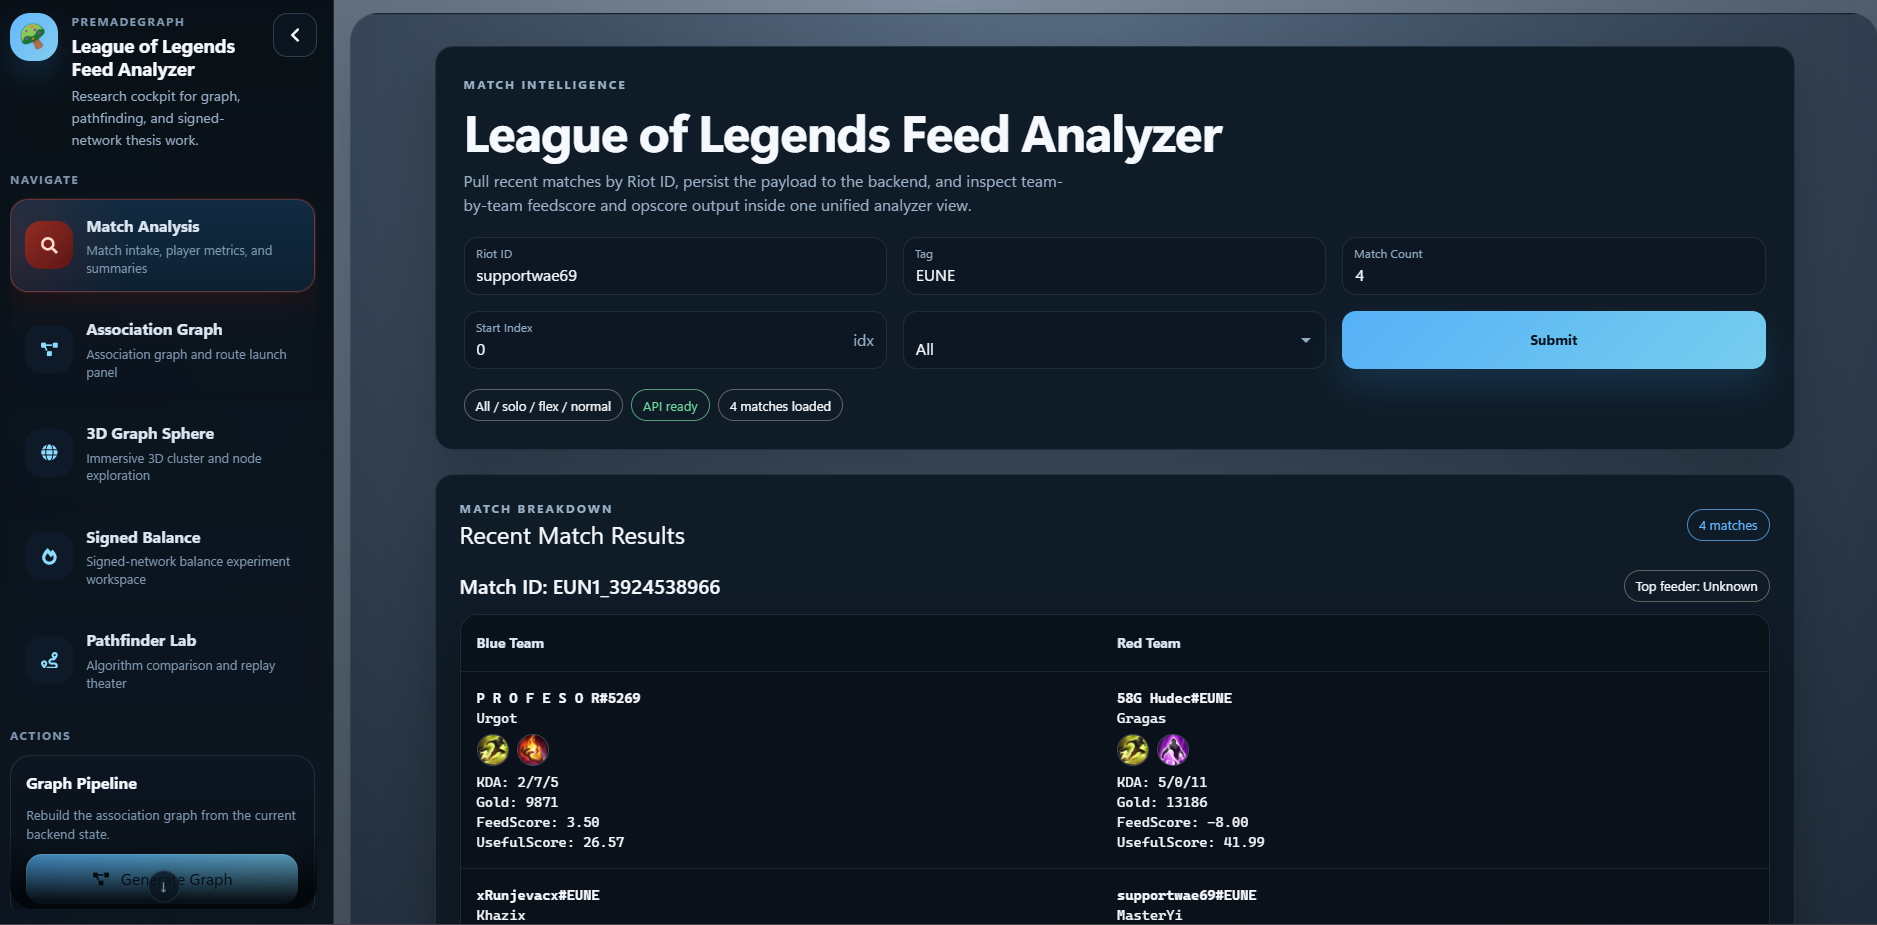
\includegraphics[width=0.92\textwidth]{match-analysis-page.png}
    \caption{A jelenlegi frontend egyik belépési pontja: meccselemzési és adatgyűjtési felület}
\end{figure}

\chapter{Problémafelvetés és motiváció}

\section{Miért nem elég egy hagyományos statisztikai oldal?}

A legtöbb, játékosoknak szánt statisztikai felület egyetlen mérkőzésre, egyetlen rangsorra vagy néhány alapmutatóra szűkíti le az értelmezést. Ez önmagában hasznos lehet, de nem válaszolja meg azt a kérdést, amely engem a projekt elejétől fogva érdekelt: vajon a mérkőzések mögött kirajzolódik-e egy tartós társas szerkezet, és ha igen, ez a szerkezet hogyan kapcsolódik a teljesítményhez?

Ebből a szempontból a \emph{Premade Graph} lényegében két problémát kezel egyszerre. Az első probléma adatmérnöki: hogyan lehet nyers Riot API válaszokból olyan hosszabb élettartamú adatkorpuszt felépíteni, amelyben a játékosok azonosítása, a meccsek tárolása, a pontszámítás és a gráfprojekció újrafuttatható módon történik. A második probléma kutatási: hogyan lehet ebből a korpuszból olyan állításokat megfogalmazni, amelyek nem csak látványosak, hanem meg is védhetők.

Ez az oka annak, hogy a dolgozat fókusza tudatosan nem egyetlen UI-oldal vagy egyetlen algoritmus. A projekt értéke éppen abban áll, hogy az adatgyűjtés, a tisztítás, a pontszámítás, a gráfépítés, a klaszterezés, a futásidejű analitika és a vizualizáció ugyanannak a rendszernek az egymásra épülő rétegei.

\section{A projekt szokatlan és érdekes volta}

A szakdolgozat témája azért különösen érdekes, mert a kiinduló adathalmaz nem egyszerű játékoslista, hanem ismétlődő interakciós háló. A rendszer ugyanazt a két játékost nemcsak egyszeri ellenfelekként látja, hanem potenciális visszatérő szövetségesként, visszatérő ellenfélként, klasztertagként, hídcsúcsként vagy egy nagyobb globális hálózat részeként is.

Ez több okból ad erős szakdolgozati alapot:

\begin{itemize}
    \item a League of Legends mérkőzésadatai elég gazdagok ahhoz, hogy valódi teljesítményprofilok legyenek számíthatók;
    \item a visszatérő együttjátszás és egymás elleni előfordulás gráfelméleti szempontból értelmezhető kapcsolatokat hoz létre;
    \item a szövetségesi és ellenfél-jelleg együttese miatt a projekt nem csak súlyozott, hanem előjeles hálózatként is vizsgálható;
    \item a rendszer implementációs oldalon is érdekes, mert több nyelv és futtatókörnyezet közötti felelősségmegosztást kell megindokolni.
\end{itemize}

Ez a kombináció ritkább, mint elsőre látszik. Sok játékelemző projekt vagy a vizuális oldalnál áll meg, vagy csak egy-egy táblázatos mutatóig jut el. Itt viszont ugyanannak a rendszernek része a nyers adatgyűjtés, a szerepkörérzékeny score-réteg, a klaszterezés, az útvonalkeresés, a signed-balance analitika és a 3D globális megjelenítés.

\section{A központi szakdolgozati állítás}

A dolgozat fő tézise az, hogy \emph{a valós mérkőzéstörténetből felépített League of Legends játékosháló egyszerre kezelhető mint társas hálózat, mint teljesítményprofilokkal dúsított adatstruktúra, és mint rendszertechnikai szempontból komoly, többnyelvű analitikai platform}. Ennek a tézisnek három pillére van.

\subsection{Hálózati pillér}

A meccsekből olyan gráf építhető, amelyben a játékosok közötti ismétlődő együttjátszás és egymás elleni előfordulás már nem véletlenszerű zajként, hanem mérhető szerkezeti mintázatként jelenik meg. Ez teszi lehetővé a klaszterezést, az útvonalkeresést, az asszortativitást és az előjeles triádelemzést.

\subsection{Metrikai pillér}

A játékosokhoz rendelhető olyan \texttt{feedscore} és \texttt{opscore}, amely nem tökéletes vagy végleges igazság, de elég értelmezhető és következetes ahhoz, hogy későbbi gráfanalitikai bemenet legyen. A szerepkörérzékeny súlyozás és a percentilis-alapú normalizáció itt nem kozmetikai döntés, hanem a teljes későbbi elemzés előfeltétele.

\subsection{Rendszertechnikai pillér}

A projekt a jelenlegi állapotában már túlmutat azon, amit egyetlen script vagy egyetlen technológia kényelmesen elbírna. A Python, az SQLite, a Node/Express, a Rust és a React együttese nem véletlen felhalmozódás, hanem olyan architekturális válasz, amely a különböző részfeladatok eltérő természetéből következik. Ezt a dolgozatban külön, döntési és kompromisszum-alapú szemlélettel fogom indokolni.

\section{Hatókör, nem-célok és őszinteségi szabályok}

A projekt mérete könnyen csábíthatna arra, hogy minden meglévő ötletet kész eredményként mutassak be. Ezt a dolgozatban tudatosan kerülöm. Három szabályt tekintek fontosnak.

\begin{itemize}
    \item Amit a kódbázisban jelenleg ténylegesen megvalósultnak és ellenőrizhetőnek találtam, azt kész állapotként írom le.
    \item Amit a repository megőriz korábbi kísérleti ágként, de a jelenlegi adatsnapshotban nincs érdemi kimenete, azt korábbi vagy kiegészítő modulként kezelem.
    \item Amit az \texttt{AGENTS.md} és a fejlesztési dokumentáció csak jövőbeli célként fogalmaz meg, azt nem nevezem kész feature-nek.
\end{itemize}

Ennek a szabálynak különösen nagy jelentősége van a következő területeken:

\begin{itemize}
    \item a klaszterekhez kötött ország- és régióelemzés kódja megvan, de a jelenlegi ellenőrzött adatbázis-pillanatképben nem tartalmaz kitöltött országcímkéket;
    \item a több-adatkészletes architektúra implementált, de a történetileg gazdag, régi \texttt{playersrefined.db} állomány migrációja a mostani repository-állapotban még nem teljesen zárult le;
    \item a párhuzamos Brandes-központiság, a temporális stabilitási mutatók, a kohézió--teljesítmény kapcsolat és az adatvezérelt \texttt{opscore}-kalibráció jelenleg jövőbeli munka.
\end{itemize}

\section{A dolgozat szerkezete}

A dolgozat logikája a projekt fejlődését követi. Előbb bemutatom a problémafelvetést és a szakirodalmi hátteret, majd a Riot API-ra épülő adatforrásokat és a korai pipeline-t. Ezután térek rá a pontozási rendszerre, a gráfépítésre és a régi ország-alapú elemzési ágra. A középső fejezetek az architektúra evolúcióját, a több-adatkészletes modellt, az SQLite perzisztenciát és a Rust futtatókörnyezetet tárgyalják. Végül külön fejezetekben mutatom be a Pathfinder Labot, a 3D bird's-eye sphere nézetet, a signed-balance és asszortativitási elemzéseket, majd a validációt, a rendszerszintű értékelést és a jövőbeli fejlesztéseket.

\chapter{Szakirodalmi háttér}

\section{Hálózatkutatás és közösségszerkezet}

A gráfok társas kapcsolatok modellezésében régóta központi szerepet játszanak. A videojátékos közösségek esetében különösen izgalmas kérdés, hogy a játékosok közötti ismétlődő interakciók mennyiben alkotnak felismerhető struktúrákat, szubközösségeket, hidakat és lokális mintázatokat. Girvan és Newman klasszikus munkája rámutatott arra, hogy a hálózat élei nem pusztán kapcsolódási elemek, hanem közösségszerkezetet leíró, eltérő fontosságú viszonyok is lehetnek \cite{girvannewman}. Fortunato átfogó áttekintése pedig jól összefoglalja, miért központi probléma a közösségdetektálás a modern hálózatelemzésben \cite{fortunato2010}.

A jelen projektben a közösségfogalom nem öncélú. Azért fontos, mert a többször ismétlődő kapcsolatokra épülő játékoscsoportok:

\begin{itemize}
    \item értelmezhetőbbé teszik a nagyméretű hálózatot,
    \item segítenek elkülöníteni a valós kapcsolati magokat a zajtól,
    \item támaszt nyújtanak a későbbi útvonal- és analitikai számításoknak.
\end{itemize}

\section{Közösségdetektálás és modularitás}

A Python oldali klaszterezés jelenleg a NetworkX \texttt{greedy\_modularity\_communities} eljárását használja, amely a Clauset--Newman--Moore féle mohó modularitásmaximalizálási megközelítésre épül \cite{clauset2004,networkx_greedy}. Ez a választás tudatos kompromisszum: nem a leglátványosabb, hanem a jelenlegi adatkészlet és pipeline mellett a legegyszerűbben magyarázható és stabilan reprodukálható megoldás.

A dolgozatban ezért nem azt állítom, hogy ez az egyetlen vagy minden helyzetben legjobb közösségdetektáló eljárás, hanem azt, hogy a jelenlegi rendszerben ez adja a legvédhetőbb kiindulópontot a közösségek strukturált tárolására és vizsgálatára.

Ugyanakkor módszertanilag fontos kimondani a modularitás-optimalizáció ismert korlátait is. Fortunato és Barthelemy klasszikus eredménye szerint a modularitásra építő közösségdetektálás felbontási korlátba ütközhet, vagyis a kisebb, de valós szerkezetek egy része a globális optimum érdekében összeolvadhat \cite{fortunato_barthelemy2007}. Ez a jelen projektben azért releváns, mert a \texttt{python\_population} klasztereket nem szabad ontológiai „igazi közösségként” kezelni. Sokkal pontosabb azt mondani, hogy a választott gráf, súlymodell és heurisztika mellett ezek adják a legjobb, reprodukálható populációs közösségképet.

Ez a szakirodalmi háttér azt is megvilágítja, miért védhető a két klasztercsalád együttélése. Ha a közösségdetektálás eleve input- és célfüggő feladat, akkor nem meglepő, hogy a populációs Python-klaszterek és a futásidejű Rust-komponensek nem esnek egybe. A dolgozat szempontjából ez nem hiba, hanem annak jele, hogy a rendszer külön optimalizálja a népességi értelmezhetőséget és a keresési használhatóságot.

\section{Strukturális egyensúly és előjeles gráfok}

Az előjeles kapcsolatok vizsgálatának klasszikus alapját Heider egyensúlyelmélete \cite{heider1946}, illetve Cartwright és Harary gráfelméleti általánosítása adja \cite{cartwright1956}. Az alapgondolat intuitív: a pozitív és negatív kapcsolatokból felépülő triádok egy része stabilabb, más része feszültebb szerkezetet jelez.

Ez a dolgozat szempontjából azért különösen fontos, mert a projekt adatmodellje nemcsak azt tudja megmondani, hogy két játékos hányszor került kapcsolatba, hanem azt is, hogy ez a kapcsolat inkább szövetségesi vagy inkább ellenfél-jellegű volt. Így a gráf természetes módon projektálható egy előjeles hálóvá, ahol:

\begin{itemize}
    \item a domináns \texttt{ally} kapcsolat pozitív élként,
    \item a domináns \texttt{enemy} kapcsolat negatív élként
\end{itemize}

jelenik meg.

A modern signed-network irodalom azért is hasznos háttér, mert rámutat: az előjeles hálók viselkedése nem csak elméleti játék. Leskovec és munkatársai nagyméretű online hálózatokon mutatták meg, hogy a pozitív és negatív élek kombinációja valódi szerkezeti mintázatokat hoz létre \cite{leskovec2010}, míg későbbi összefoglalók és empirikus vizsgálatok azt hangsúlyozzák, hogy a strukturális egyensúlyt mindig a konkrét projekciós szabályok és adatkeletkezési mód fényében kell értelmezni \cite{lerner2016,facchetti2011}.

\section{Asszortativitás}

Newman munkája az asszortatív keveredést olyan hálózati jelenségként írja le, amikor a kapcsolódó csomópontok hasonló vagy éppen eltérő tulajdonságúak \cite{newman2003}. A jelen projektben ezt a gondolatot a játékosok teljesítménymutatóira alkalmazom: nem azt kérdezem, hogy a magas fokszámú csúcsok kapcsolódnak-e egymáshoz, hanem azt, hogy a gráfban összekapcsolt játékosok hasonló \texttt{opscore} vagy \texttt{feedscore} értékeket hordoznak-e.

Ez azért különösen hasznos, mert:

\begin{itemize}
    \item könnyen értelmezhető,
    \item számszerűsíthető,
    \item a gráf jelentésétől függően más és más eredményt adhat.
\end{itemize}

Éppen ezért a dolgozatban két gráfmódot is megkülönböztetek:

\begin{itemize}
    \item \texttt{social-path}: csak a pozitív, szövetségesi támaszú kapcsolatokra épít,
    \item \texttt{battle-path}: az összes ismétlődő együtt- vagy egymás ellen játszást figyelembe veszi.
\end{itemize}

\section{Legrövidebb utak és heurisztikus keresés}

A gráfok másik természetes vizsgálati iránya az útvonalak keresése. A klasszikus legrövidebb út problémát Dijkstra alapozta meg \cite{dijkstra1959}, míg az A* keresés formális alapját Hart, Nilsson és Raphael adták meg \cite{hart1968}. A jelen projektben azért vált ez fontos kérdéssé, mert a játékosháló nemcsak statikus objektumként érdekes, hanem úgy is, mint egy olyan kapcsolati tér, ahol két játékos között különböző „ismeretségi láncok” húzódhatnak.

A Rust rétegben bevezetett egzakt A* implementációhoz a rendszer ALT-szerű alsó becsléseket is használ, amelyeket a Goldberg--Harrelson-féle irány tovább inspirált \cite{goldberg2005}. A lényeg itt sem az, hogy a dolgozat egy új legrövidebb út algoritmust találna fel, hanem az, hogy a játékosháló nagyságrendjéhez és a demo-igényekhez illeszkedően stabil, védhető és gyors futtatókörnyezetet alakítson ki.

Szakdolgozati szempontból itt különösen fontos különbséget tenni „gyorsnak tűnő” és valóban helyes heurisztikus keresés között. Sok gyakorlati rendszer a képernyőn látható távolságot is heurisztikaként használja, ami látványos lehet, de nem feltétlenül admisszibilis. A jelen projektben a helyességi garancia nem a layoutból, hanem a gráfra illesztett alsó becslésekből származik. A térbeli távolság legfeljebb tie-break szerepet kap. Ezzel a rendszer jobban igazodik a klasszikus A* elméleti követelményeihez, és elkerüli, hogy a vizualizációs koordináták összekeveredjenek a kapcsolati költséggel.

\chapter{Riot API, adatforrások és adatgyűjtési stratégia}

A rendszer elsődleges adatforrása a Riot Developer Portal és a kapcsolódó League of Legends API-készlet \cite{riotportal,riotapi}. Ezek lehetővé teszik:

\begin{itemize}
    \item játékosfiókok azonosítását,
    \item meccslisták lekérdezését,
    \item részletes meccs-JSON-ok letöltését,
    \item résztvevői statisztikák és szerepkörök feldolgozását.
\end{itemize}

Az API ugyanakkor nem korlátlan: a fejlesztői kulcsok szigorú sebességkorlátokkal működnek, és ezek az architektúrát is befolyásolják. Ez magyarázza, hogy a projektben miért különül el világosan az adatgyűjtő, a normalizáló, a gráfépítő és a futtatókörnyezeti réteg. A cél ugyanis nem az, hogy minden egyszerre, ugyanabban a kérésben történjen, hanem az, hogy a rendszer különálló, újrafuttatható lépésekből álljon össze.

\section{A használt Riot API-végpontok logikája}

A jelenlegi projekt a Riot API több rétegét használja, de a legfontosabb tervezési döntés az volt, hogy a rendszer központi azonosítójává a \texttt{puuid} váljon. Ez a döntés végigvonul az egész kódbázison. A felhasználóbarát név és tag ugyan hasznos a frontendben, de az adatbázis és a gráfépítés szempontjából az azonosíthatóság elsődleges.

A pipeline logikailag az alábbi lépésekre bontható:

\begin{enumerate}
    \item egy kiinduló játékos vagy seed-lista alapján a rendszer fiókinformációt kér le;
    \item a fiókból meccsazonosító-listát szerez;
    \item a meccsazonosítókhoz letölti a részletes match JSON-okat;
    \item a résztvevői sorokból \texttt{puuid}-alapú játékosprofilt és kapcsolati adatot képez;
    \item az eredményt datasethez kötve perzisztálja.
\end{enumerate}

Ez azért szerencsés, mert a névváltozások, régiós sajátosságok és meccslistás lekérdezések nem keverednek össze a későbbi gráf- és pontszámítási lépésekkel. A \texttt{puuid} egyszerre stabil összekötő kulcs a nyers meccsadat, a játékosprofil és a gráfcsúcs között.

\subsection{Régiós routing és végpont-topológia}

A konkrét implementáció szintjén ez a logika azt is jelenti, hogy a meccslisták és a részletes meccsadatok a region routing logikát követik. A jelenlegi collector a \texttt{match-v5} végpontokat az \texttt{europe.api.riotgames.com} címen keresztül hívja. Ez első látásra technikai apróságnak tűnhet, de a teljes adatgyűjtési megbízhatóság múlik rajta: hibás routing mellett a rendszer úgy tűnhet működőképesnek, hogy közben a lekérdezések egy része konzisztensen elbukik.

\begin{table}[H]
\centering
\caption{A gyűjtőréteg fő végpontjai és szerepük}
\begin{tabularx}{\textwidth}{>{\raggedright\arraybackslash}p{4.4cm}X}
\toprule
\textbf{Végpontcsalád vagy réteg} & \textbf{Szerep a pipeline-ban} \\
\midrule
Fiók- és seed-feloldás & Kiinduló játékosok azonosítása és stabil kulcshoz kötése \\
\texttt{/lol/match/v5/matches/by-puuid/\{puuid\}/ids} & Meccsazonosítók lekérése egy adott játékoshoz \\
\texttt{/lol/match/v5/matches/\{matchId\}} & A teljes meccs-JSON letöltése minden résztvevő adattal \\
Lokális normalizálás & A letöltött JSON-ból PUUID-alapú játékosprofil és későbbi gráfinput képzése \\
\bottomrule
\end{tabularx}
\end{table}

Az architekturális tanulság az, hogy a külső, kvótás réteget minél hamarabb érdemes lokális állapottá alakítani. A rendszer ezért a külső API-hívásokat csak a nyers meccs-JSON-ig viszi, utána a feldolgozás már lokális fájlokon és adatbázison történik.

\subsection{Collector állapotgép és premade-probe}

A \texttt{backend/match\_collector.py} vizsgálata alapján a collector nem egyszerű lineáris letöltőszkript, hanem paraméterezhető állapotgép. A konfiguráció tartalmazza többek között a \texttt{datasetId}, \texttt{rawDbPath}, \texttt{matchesDir}, \texttt{collectorMode}, \texttt{queueType}, \texttt{matchesPerPlayer}, \texttt{maxIterations}, \texttt{probeMatchCount} és \texttt{minimumPremadeRepeats} mezőket. Ennek következtében a gyűjtés explicit módon szabályozható, újrafuttatható és különböző célokra hangolható.

A tipikus futás így írható le:

\begin{enumerate}
    \item a backend kijelöli az aktív datasetet és előkészíti az útvonalakat;
    \item a collector véletlen vagy konkrét \texttt{puuid} alapján jelölt játékost választ;
    \item rövid meccslista-lekéréssel premade-probe történik;
    \item ha a jelölt elég ismétlődő csapattársi mintázatot mutat, teljesebb gyűjtés indul;
    \item a letöltött meccsek eseményes logolás mellett fájlba kerülnek;
    \item az eredmény később normalizáló és gráfépítő pipeline-ba lép tovább.
\end{enumerate}

Ez a részlet azért fontos, mert a premade-fókusz nem csak a későbbi gráfelemzés szintjén jelenik meg, hanem már a mintavételi mechanizmusban is. A rendszer tehát nem utólag próbálja kiszűrni a visszatérő kapcsolatok jelentőségét, hanem a gyűjtési stratégiát is erre hangolja.

\section{Gyűjtési fókusz és queue-választás}

A rendszer nem a Riot teljes játékuniverzumát próbálja egyetlen adatfolyamba összesöpörni, hanem tudatosan olyan queue-típusokból építkezik, amelyekben az ismétlődő kapcsolatok és a premade-jelleg reálisabban megjelenhet. Ez az oka annak, hogy a repository dokumentációja és gyűjtőszkriptjei külön foglalkoznak az EUNE és a Master/SoloQ jellegű mintákkal, illetve a gyors tesztadatsorokkal.

A 2026. április 24-én ellenőrzött \texttt{default} dataset queue-eloszlása a következő volt:

\begin{table}[H]
\centering
\caption{Queue-eloszlás az aktív \texttt{default} dataseten}
\begin{tabular}{lrr}
\toprule
\textbf{Queue ID} & \textbf{Darabszám} & \textbf{Értelmezés} \\
\midrule
420 & 1371 & Ranked Solo/Duo \\
440 & 1351 & Ranked Flex \\
450 & 358 & ARAM \\
400 & 313 & Normal Draft \\
900 & 45 & URF / rotációs mód \\
480 & 20 & Normal Blind \\
700 & 9 & Clash \\
740 & 2 & Intro/AI jellegű mód \\
870 & 2 & Egyéb speciális queue \\
\bottomrule
\end{tabular}
\end{table}

Ez két fontos dolgot jelez. Egyrészt a korpusz zöme olyan játékmódból jön, ahol a kompetitív ismétlődés reális. Másrészt a dataset vegyes: a rangsorolt játékon kívül ARAM és normál draft elemek is bekerültek. Emiatt a dolgozatban különösen fontos, hogy a gráfot ne „barátsági gráfként”, hanem ismétlődő játékkapcsolati hálóként kezeljem.

\begin{table}[H]
\centering
\caption{Térképeloszlás az aktív \texttt{default} dataseten}
\begin{tabular}{lrr}
\toprule
\textbf{Map ID} & \textbf{Darabszám} & \textbf{Értelmezés} \\
\midrule
11 & 3113 & Summoner's Rift \\
12 & 358 & Howling Abyss \\
\bottomrule
\end{tabular}
\end{table}

A map-eloszlás azt is mutatja, hogy a korpusz döntően a klasszikus Summoner's Rift környezetre épül. Ez azért lényeges, mert a szerepkörök, az útvonalkeresési interpretáció és a teljesítménymutatók is ebben a közegben a legjobban értelmezhetők.

\section{Premade-fókusz és gyűjtési stratégiai intuíció}

A projekt mögött végig ott állt az a gyakorlati intuíció, hogy az igazán érdekes kapcsolatok nem az egyszeri, véletlenszerű találkozásokból születnek, hanem a visszatérő együtt- vagy egymás ellen játszásból. Emiatt a gyűjtőszkriptek és a dokumentáció egy része kifejezetten premade-szerű vagy ismétlődő kapcsolatok felderítésére van hangolva.

Ez a szemlélet a teljes későbbi rendszerre hatással volt:

\begin{itemize}
    \item a gráfépítésben élküszöb jelent meg;
    \item a signed-balance az ismétlődő kapcsolatokat tekinti komoly jelöltnek;
    \item a pathfinder-költségek is a kapcsolaterősséget veszik figyelembe.
\end{itemize}

Másképp fogalmazva: a gyűjtési stratégia nem előszoba, hanem a későbbi gráfjelentés egyik meghatározó forrása.

Ez a döntés ugyanakkor tudatos torzítást is bevezet. Ha a gyűjtés a visszatérő, premade-szerű kapcsolatokat részesíti előnyben, akkor a korpusz kevésbé reprezentálja az egyszeri és lazább találkozásokat. A jelen dolgozat céljai mellett ez elfogadható kompromisszum, mert a kutatási kérdés középpontjában éppen a tartósabb kapcsolati magok állnak. A háló tehát nem a teljes populáció semleges lenyomata, hanem az ismétlődő interakciók felé célzottan dúsított részvilág.

\section{Rate limit, megbízhatóság és operatív kompromisszumok}

A Riot API használata az architektúrában nem pusztán külső függőség, hanem korlátozó tényező is. A fejlesztői kulcsok lekérdezésszámhoz kötöttek, ezért a gyűjtőrétegben explicit sebességkorlát-kezelés, várakozási logika és részfeladatokra bontás jelent meg. A dokumentációban rögzített rate-limit elemzés ezt nem adminisztratív részletként, hanem rendszertervezési kényszerként kezeli.

Ennek közvetlen következményei:

\begin{itemize}
    \item a meccsletöltés nem kérésenkénti frontend-akcióként, hanem háttérfolyamatként fut;
    \item a nyers adatállapotot érdemes lokálisan cache-elni;
    \item a grafikus és analitikai oldal nem függhet attól, hogy egy élő API-lekérés éppen sikeres-e.
\end{itemize}

Ez a döntés később az egész rendszer egyik alapelve lett: \emph{a demo- és kutatási réteg a már összegyűjtött korpuszra épül, nem online API-kérésekre}.

Az implementáció szintjén ez több konkrét védelmet jelent. A collector saját másodpercenkénti várakozást alkalmaz, külön kétperces ablakban számlálja a kéréseket, \texttt{HTTP 429} esetén harminc másodpercet vár, majd újrapróbálkozik, és a már elmentett meccseket fájllétezés alapján kihagyja. Ez a működés idempotenssé teszi a letöltést: egy megszakadt vagy újraindított futás nem írja felül feleslegesen a korábbi állományokat, és nem épít újabb bizonytalanságot a nyers korpuszba.

\begin{table}[H]
\centering
\caption{A collector fő megbízhatósági mechanizmusai}
\begin{tabularx}{\textwidth}{>{\raggedright\arraybackslash}p{4.4cm}X}
\toprule
\textbf{Mechanizmus} & \textbf{Funkció} \\
\midrule
Saját \texttt{requestsPerSecond} késleltetés & A rövid távú API-terhelés kontrollja \\
Kétperces számláló & Illeszkedés a Riot kulcshasználati limitjeihez \\
\texttt{429} újrapróbálás & Robusztusabb működés átmeneti limitütközéskor \\
Létező meccsfájl kihagyása & Duplikált mentés és újra-letöltés elkerülése \\
Eseményes stdout log & Backend- és frontend-oldali állapotkövetés támogatása \\
\bottomrule
\end{tabularx}
\end{table}

Ezek a döntések nem puszta üzemeltetési kényelmi funkciók. A reprodukálható számítógépes kutatás egyik alapelve, hogy az eredményekhez vezető lépések nyomon követhetők és lehetőleg automatizálhatók legyenek \cite{sandve2013}. A collector parametrizálhatósága, eseményes logolása és idempotens mentési logikája pontosan ezt a célt szolgálja.

\section{Adatminőség, torzítás és óvatos interpretáció}

A Riot API formálisan pontos, de a dolgozat szempontjából az adat így sem „semleges”. A mintavételt erősen befolyásolja:

\begin{itemize}
    \item milyen seed játékosokról indult a gyűjtés;
    \item mely queue-k kerültek előtérbe;
    \item milyen mélyre ment a meccslista-lekérés;
    \item a premade-kapcsolatok milyen minimumismétlés után tekinthetők érdekesnek.
\end{itemize}

Ezért a dolgozat minden későbbi eredményénél fontos megjegyzés, hogy a hálózat \emph{nem a teljes League of Legends univerzum reprezentációja}, hanem egy adott gyűjtési stratégia által létrehozott, vizsgálható részvilág. Ez nem gyengeség, hanem korrekt keretfeltétel.

További torzításforrás, hogy a dataset fokozatosan épülő archívumként működik. A meccsek nem egyetlen, szigorúan lezárt időablakból származnak, ezért a játékosok \texttt{match\_count} értékei részben azt is tükrözik, mennyire került rájuk fókusz a gyűjtési folyamatban. Emiatt a score-réteg és az időbeliség kapcsolatát mindig óvatosan kell kezelni: a magasabb mintaszám nem kizárólag aktivitást, hanem gyűjtési figyelmet is jelenthet.

\chapter{A rendszer korai változata és az eredeti pipeline}

\section{A korai projekt jellege}

A repository története alapján a rendszer első változata jóval közelebb állt egy adatvezérelt játékosnézőhöz és kísérleti gráf-exportáló eszközhöz, mint a jelenlegi, több rétegre bontott kutatási platformhoz. Ebben a szakaszban a cél elsősorban az volt, hogy:

\begin{itemize}
    \item a Riot API-ból érkező nyers mérkőzésadatok egy helyre kerüljenek;
    \item a játékosokhoz legalább alapvető pontszámok rendelődjenek;
    \item a kapcsolatokból egyszerű gráf és klaszterkimenet szülessen;
    \item a projekt vizuálisan is megmutatható legyen.
\end{itemize}

Ez a korai szakasz nem eldobandó előtörténet, hanem a jelenlegi rendszer kiindulópontja. A dolgozatban azért tartom meg hangsúlyosan, mert ebből érthető meg, miért alakult ki később a többnyelvű architektúra és a szigorúbb perzisztenciamodell.

\section{Az első pontozási logika}

Az eredeti \texttt{add\_new\_players.js} egyszerűbb, kézzel összeállított képletekkel dolgozott. A korai \texttt{feedscore} lényegében a halálokat büntette a kill és assist mennyiségéhez képest, míg az első \texttt{opscore} főként a következő komponensekre támaszkodott:

\begin{itemize}
    \item ölések,
    \item asszisztok,
    \item arany,
    \item vision score.
\end{itemize}

Ez a kezdeti modell nyers volt, de fontos előnye volt: gyorsan megmutatta, hogy a tiszta KDA-logikán túl is lehet értelmes, legalább részben kompozit teljesítménymutatót számolni. Később ebből nőtt ki az artifact-szintű és szerepkörérzékeny rendszer.

\section{A korai gráfépítés és export}

A korai \texttt{build\_graph.py} és a hozzá kapcsolódó exportlépések alapvetően Python-központúak voltak. A hangsúly ekkor még a gyors láthatóságon és nem a perzisztens újrafelhasználhatóságon volt. A pipeline:

\begin{itemize}
    \item meccsekből kapcsolati gráfot épített,
    \item összefüggő komponenseket és részgráfokat vizsgált,
    \item HTML és PyVis exportokat készített,
    \item gyors vizuális ellenőrzést tett lehetővé.
\end{itemize}

Ez a megközelítés jó prototípus volt, de rövid időn belül látszott a korlátja: a klaszterek és gráfnézetek csak exportként éltek tovább, és nem váltak a rendszer belső, lekérdezhető objektumaivá.

\section{A korábbi régiós és ország-alapú ág kialakulása}

A projekt korai időszakában erősebb szerepet kapott az a gondolat is, hogy a klaszterekből ország- vagy régiószintű következtetések szülessenek. Ennek nyomai ma is megtalálhatók a \texttt{fetch\_clusters.py}, \texttt{assign\_countries.py} és \texttt{conclude.py} szkriptekben. A megközelítés lényege az volt, hogy a klaszterek tagneveiből valamilyen földrajzi címke becsülhető, majd ehhez aggregált teljesítményadatok rendelhetők.

Ez a gondolat önmagában izgalmas, de a dolgozat mostani állapotában már világos, hogy módszertanilag bizonytalanabb, mint a közvetlenül a gráfstruktúrára és a meccsadatokra támaszkodó elemzések. Emiatt ezt a vonalat nem törlöm ki a történetből, hanem kifejezetten korábbi, exploratív modulként kezelem.

\section{Miért kellett a rendszert továbbépíteni?}

A korai változat legfontosabb korlátai a következők voltak:

\begin{itemize}
    \item egyetlen adatbázis és egyetlen meccskönyvtár köré szerveződött;
    \item a klaszterek és exportok nem voltak igazán első osztályú perzisztens objektumok;
    \item a pontozás még nem volt kellően szerepkörérzékeny;
    \item a futásidejű útvonalkeresés és a nehezebb gráfanalitika nem vált el élesen a frontend-logikától.
\end{itemize}

Ezek a hiányok nem kudarcot jeleztek, hanem természetes érési pontokat. A jelenlegi rendszer legjobban akkor érthető, ha nem egyetlen pillanatfelvételként, hanem ilyen fokozatos evolúció eredményeként nézzük.

\section{Miért kellett a régi szövegréteget is megtartani?}

Szakdolgozatírás közben könnyű lenne azt a hibát elkövetni, hogy a projekt korábbi állapotát egyszerűen ``lecserélem'' a jelenlegi, erősebb verzióra. Ezt tudatosan nem teszem. A korai pipeline, a \texttt{conclude.py}-szerű ág és a régi klaszterértelmezések azért maradnak a dolgozatban, mert ezek adják meg a fejlődés irányát. A mostani rendszer nem légüres térben született, hanem ezekből nőtt ki.

\diagramfigure{Tevékenységdiagram a korai adatgyűjtő és gráfépítő pipeline-hoz}{activity diagram.pdf}

\chapter{A rendszerarchitektúra evolúciója}

\section{Áttekintés}

A projekt jelenlegi architektúrája tudatosan hibrid. Első ránézésre ez bonyolultabbnak tűnhet, mint egyetlen nyelvre vagy egyetlen futtatókörnyezetre építeni mindent, de a jelen esetben éppen ez a szétválasztás teszi védhetővé a rendszert.

A feladat ugyanis több, egymástól eltérő természetű részre oszlik:

\begin{itemize}
    \item adatgyűjtés és tömeges JSON-feldolgozás;
    \item statisztikai és szerepkör-érzékeny pontszámítás;
    \item gráfépítés és klaszterezés;
    \item futási időben használható, gyors útvonalkeresés és analitika;
    \item böngészőben is jól prezentálható vizualizáció.
\end{itemize}

Ezeket a projekt az alábbi rétegek között osztja szét:

\begin{itemize}
    \item \textbf{Python}: gyűjtés, gráfépítés, közösségdetektálás, exportfolyamatok;
    \item \textbf{SQLite}: központi perzisztens tárolás;
    \item \textbf{Node.js / Express}: API-héj és orchesztráció;
    \item \textbf{Rust}: útvonalkeresés, előjeles analitika, globális gráf-artifaktumok;
    \item \textbf{React + Vite}: interaktív frontend és vizuális prezentáció.
\end{itemize}

\diagramfigure{Komponensdiagram a jelenlegi rendszerhez}{component diagram.pdf}

\section{Miért nem egyetlen technológia?}

A rendszer felépítésében a legfontosabb architekturális elv az volt, hogy \emph{a kontextus dönti el a technológiát}, nem fordítva. A Python kiváló az adatgyűjtéshez, a JSON-feldolgozáshoz és a hálózatépítés gyors iterációjához. A Rust viszont sokkal alkalmasabb a nagyméretű, ismételten meghívott gráfalgoritmusokhoz, ahol fontos a determinisztikus viselkedés, a teljesítmény és a strukturált export. Az SQLite kis projektméret mellett is kényelmesen biztosítja a perzisztenciát, a React pedig jó eszköz a demo- és elemzőfelületek építéséhez.

Ez a szétválasztás nem „tech stack gyűjtögetés”, hanem tudatos munkamegosztás:

\begin{itemize}
    \item az adatfeldolgozó lépések külön újrafuttathatók,
    \item a számításigényes részek nincsenek a böngészőre tolva,
    \item az eredményeket tárolni, exportálni és később újrafelhasználni is lehet.
\end{itemize}

\subsection{Elvetett architekturális alternatívák}

Az \texttt{architecture-decision} szemlélet szerint nem csak a végső döntést, hanem az elutasított alternatívákat is érdemes dokumentálni. A projekt fejlődése során legalább négy természetes irány merülhetett volna fel:

\begin{table}[H]
\centering
\caption{Fontos architekturális alternatívák és elutasításuk oka}
\begin{tabularx}{\textwidth}{>{\raggedright\arraybackslash}p{3.5cm} >{\raggedright\arraybackslash}p{3.6cm} X}
\toprule
\textbf{Alternatíva} & \textbf{Rövid előny} & \textbf{Miért nem ez lett a végső irány?} \\
\midrule
Minden Pythonban & Gyorsabb kezdeti iteráció & A futásidejű gráfalgoritmusoknál és a nagyobb exportoknál gyengébb teljesítmény- és memóriakontroll \\
Minden Rustban & Erős típusosság és egységes motor & A gyűjtés és a gyors kísérletezés jelentősen nehezebbé és lassabbá vált volna \\
Frontend-központú számítás & Egyszerűbb demoarchitektúra & A böngészőre tolta volna a számításigényes gráfmunkát, gyengítve a reprodukálhatóságot \\
Szerveres SQL-adatbázis & Erősebb többfelhasználós modell & A projekt lokális, bemutatható és kutatásorientált természete mellett az SQLite kedvezőbb kompromisszum maradt \\
\bottomrule
\end{tabularx}
\end{table}

Különösen fontos itt a Python és Rust közti munkamegosztás. A Python megőrizte a gyors adatmanipuláció és prototípuskészítés előnyeit, míg a Rust a stabil futásidejű gráfmag szerepét kapta. A kettő közé a Node/Express réteg került, amely szerződéses API-határként működik.

\subsection{Miért maradt a Node középen?}

Felmerülhetne, hogy a frontend miért nem közvetlenül a Rust motorral kommunikál, vagy miért nem a Python szolgálja ki a teljes alkalmazást. A \texttt{backend/server.js} alapján a Node rétegnek önálló felelőssége van:

\begin{itemize}
    \item dataset-regisztert kezel és aktív datasetet választ;
    \item futás közbeni kulcsokat és környezeti útvonalakat központosít;
    \item háttércollector folyamatokat indít és monitoroz;
    \item HTTP-végpontokat biztosít a Rust parancsok fölé;
    \item a bird's-eye artifaktumokat és egyéb cache-eket konzisztensen szolgálja ki.
\end{itemize}

Ez a köztes réteg csökkenti a frontend és a számítási mag közti csatolást. A böngészőnek nem kell folyamatindítással, fájlrendszer-útvonalakkal vagy dataset-propagálással foglalkoznia; ezek a backendben maradnak.

\section{Evolúciós fázisok és architekturális kompromisszumok}

Az architektúra fejlődését három, viszonylag jól elkülöníthető fázisban lehet leírni.

\begin{enumerate}
    \item \textbf{Korai script-fázis}: a hangsúly a nyers adat begyűjtésén, a gyors score-számításon és a kezdeti gráfexporton volt.
    \item \textbf{Perzisztens pipeline-fázis}: megjelent az igény arra, hogy a klaszterek és játékosprofilok ne csak pillanatnyi exportként, hanem visszatölthető adatstruktúraként éljenek tovább.
    \item \textbf{Kutatási platform-fázis}: a Rust analitika, a multi-dataset modell és a külön research oldalak megjelenésével a projekt már nem csak vizualizációs eszköz, hanem kísérleti környezet lett.
\end{enumerate}

Az \texttt{architecture-decision} szemlélet szerint minden fázisban más minőségi attribútum került előtérbe. Először a fejlesztési sebesség, utána a reprodukálhatóság, végül a teljesítmény és az elemzési mélység. Ez segít megérteni, miért nem ``inkonzisztencia'' a több réteg, hanem a rendszer természetes evolúciója.

\section{Több-adatkészletes architektúra}

A korábbi, egyetlen adatbázisra és egyetlen meccsmappára épülő modell helyett a jelenlegi rendszer már több, egymástól független adatkészletet támogat. A \texttt{backend/data/datasets.json} regiszter alapján minden dataset külön rendelkezik:

\begin{itemize}
    \item nyers adatbázissal,
    \item finomított adatbázissal,
    \item meccs-JSON könyvtárral,
    \item cache könyvtárral.
\end{itemize}

A dolgozat írásakor az aktív dataset a \texttt{default} azonosítójú alap-adatkészlet volt, de a regiszterben a \texttt{smoke-test-dataset} és a \texttt{flexset} is szerepel. Ez fontos előrelépés a korábbi állapothoz képest, mert lehetővé teszi, hogy különböző mintákon, különböző gyűjtési stratégiákkal is fusson ugyanaz az analitikai pipeline.

\begin{table}[H]
\centering
\caption{A több-adatkészletes architektúra logikai elemei}
\begin{tabularx}{\textwidth}{>{\raggedright\arraybackslash}p{3.2cm}X}
\toprule
\textbf{Elem} & \textbf{Szerep} \\
\midrule
Dataset registry & Az elérhető adatkészletek metaadatait és az aktív dataset kijelölését tárolja \\
Raw database & A gyűjtéshez és kezdeti beolvasáshoz szükséges játékosadatok \\
Refined database & A normalizált pontszámokat, klasztereket és származtatott mezőket tartalmazza \\
Matches directory & A tényleges meccs-JSON állományok helye \\
Cache directory & Futás közbeni vagy előre generált artifaktumok tárolása \\
\bottomrule
\end{tabularx}
\end{table}

\subsection{A dataset mint életciklus-egység}

A dataset a jelenlegi rendszerben nem statikus mappát, hanem együtt mozgó állapotcsomagot jelent. Egy új dataset létrehozása után több, egymástól elválasztható fázison mehet keresztül:

\begin{enumerate}
    \item nyers seed és játékosállapot kialakítása;
    \item match collector futtatása;
    \item PUUID-alapú normalizálás és score-frissítés;
    \item Python gráfépítés és klaszterperzisztencia;
    \item Rust runtime-felépítés és bird's-eye export;
    \item kutatási analitikák lefuttatása.
\end{enumerate}

Ez a bontás a dolgozat szempontjából azért erős, mert világos köztes állapotokat ad. Egy signed-balance futtatásnak nem kell újra elindítania a Riot API-gyűjtést, és egy klaszterezési változtatásnak sem kell a teljes pipeline-t újraépítenie. A dataset tehát a reprodukálható munkafolyamat egységeként is értelmezhető.

\section{A jelenlegi adatállapot}

Az aktív adatállapotot 2026. április 24-én közvetlenül a repository aktuális állapotából ellenőriztem. Ekkor:

\begin{itemize}
    \item az aktív \texttt{default} dataset könyvtárban \textbf{3471} meccs-JSON állomány szerepelt;
    \item a fő, finomított adatbázis \textbf{25\,618} játékost tartalmazott;
    \item a Python klaszterpipeline \textbf{271} darab \texttt{python\_population} klasztert tárolt;
    \item a Rust futtatókörnyezet \textbf{269} darab \texttt{rust\_pathfinding} klasztert perzisztált;
    \item a \texttt{cluster\_members} tábla \textbf{3227} tagsági rekordot tartalmazott.
\end{itemize}

Ez a pont fontos: a jelen dolgozat nem hipotetikus rendszert ír le, hanem egy olyan állapotot, amelyben a pipeline már nem csak tervekből áll, hanem futó adatokkal és konkrét kimenetekkel rendelkezik.

\diagramfigure{Adatáramlási diagram a gyűjtéstől a frontendig}{dataflow diagram.pdf}

\section{Perzisztencia és relációs modell}

A projekt egyik legfontosabb érése az volt, hogy a klaszterek kikerültek a „csak JSON export” kategóriából, és első osztályú adatbázis-objektumokká váltak. A jelenlegi séma központi táblái az SQLite perzisztenciára épülnek \cite{sqlite}:

\begin{itemize}
    \item \texttt{players},
    \item \texttt{clusters},
    \item \texttt{cluster\_members}.
\end{itemize}

A \texttt{players} tábla nemcsak a név- és országmezőket, hanem a normalizált \texttt{opscore}, \texttt{feedscore}, szerepkör, meccsszám és artifact-szintű részeredményeket is tárolja. A \texttt{clusters} és \texttt{cluster\_members} páros pedig lehetővé teszi, hogy ugyanazon játékoshoz többféle klasztertípus (\texttt{python\_population}, \texttt{rust\_pathfinding}) is kötődjön.

\diagramfigure{Relációs modell a klaszter- és játékosperzisztenciához}{relational model diagram.pdf}

\chapter{Több-adatkészletes architektúra}

\section{Miért vált szükségessé a dataset-regiszter?}

Az egyetlen adatbázisos modell korai prototípushoz még elegendő volt, de amint a projekt egyszerre kezdett demo-, smoke-test- és kutatási célokat szolgálni, világossá vált, hogy a különböző minták szétválasztása nélkül a rendszer nehezen reprodukálható. Ugyanaz a frontend, ugyanaz a Rust futtatókörnyezet és ugyanaz a Python pipeline más eredményt adhat, ha eltérő bemeneti korpuszon fut. Ezt a különbséget nem rejtett konfigurációs fájlokban, hanem explicit dataset-regiszterben érdemes kezelni.

A \texttt{backend/data/datasets.json} pontosan ezt a feladatot látja el. A dataset fogalma a jelenlegi rendszerben nem csak annyit jelent, hogy ``másik mappa'', hanem egy teljes, együtt mozgó adategységet:

\begin{itemize}
    \item nyers adatbázissal,
    \item finomított adatbázissal,
    \item meccs-JSON könyvtárral,
    \item cache-könyvtárral,
    \item megjeleníthető metaadatokkal.
\end{itemize}

\section{A jelenlegi regiszterben szereplő adatkészletek}

A dolgozat írásakor a regiszterben három dataset szerepelt:

\begin{itemize}
    \item \texttt{default},
    \item \texttt{smoke-test-dataset},
    \item \texttt{flexset}.
\end{itemize}

Az aktív dataset a \texttt{default} volt. A másik két bejegyzés jelenléte még akkor is fontos, ha a repository-pillanatképben ezek üresebbek vagy részlegesek. Ez mutatja, hogy az architektúra nem egyszeri exportfolyamatra, hanem több különböző futtatási kontextusra lett előkészítve.

\begin{table}[H]
\centering
\caption{A dataset-regiszter funkcionális szerepei}
\begin{tabularx}{\textwidth}{>{\raggedright\arraybackslash}p{4.2cm}X}
\toprule
\textbf{Funkció} & \textbf{Jelentőség} \\
\midrule
Aktív dataset kijelölése & Meghatározza, hogy a backend és a frontend mely adatkorpuszt használja alapértelmezetten \\
Eltérő tárolási útvonalak & Megakadályozza, hogy a teszt- és főadatok összekeveredjenek \\
Külön cache-ek & A bird's-eye és egyéb előre generált artifaktumok elkülönülnek \\
Kísérleti összevethetőség & Azonos pipeline különböző mintákon is futtatható \\
\bottomrule
\end{tabularx}
\end{table}

\section{A dataset-választás propagálása a backend és a Rust felé}

A dataset-ek architektúrájának egyik legfontosabb technikai előnye az, hogy a választás nem áll meg a Node-szinten. A backend a kiválasztott datasetből környezeti változókat és útvonalakat képez a Rust futtatókörnyezet felé is, például:

\begin{itemize}
    \item \texttt{DATASET\_ID},
    \item \texttt{GRAPH\_DB\_PATH},
    \item \texttt{PATHFINDER\_MATCH\_DIR},
    \item \texttt{PATHFINDER\_BIRDSEYE\_CACHE\_DIR}.
\end{itemize}

Ez építészetileg nagyon fontos döntés. Nincs külön ``frontend igazság'', ``backend igazság'' és ``Rust igazság'' ugyanarról az adatállapotról: a dataset-választás a teljes végrehajtási láncon végigmegy.

A \texttt{server.js} szintjén ez úgy valósul meg, hogy a szerver a kiválasztott datasetből egységes környezeti változókészletet képez, például \texttt{DATASET\_ID}, \texttt{GRAPH\_DB\_PATH}, \texttt{PATHFINDER\_MATCH\_DIR} és \texttt{PATHFINDER\_BIRDSEYE\_CACHE\_DIR} formában. A Rust runtime ezeket fogyasztja, így a teljes végrehajtási lánc ugyanarra az adatvilágra áll rá. Ez különösen fontos a védhetőség szempontjából: a frontend által mutatott eredmény nem különálló demonstrációs adatból, hanem ugyanabból a datasetből jön, amelyen a kutatási analitika is fut.

\section{Őszinte állapotkép a migrációról}

A több-adatkészletes architektúra implementált, de a repository ellenőrzött pillanatképe alapján a történetileg gazdagabb \texttt{playersrefined.db} állomány még nem teljesen simult bele a dataset-könyvtárstruktúrába. A vizsgálat során az látszott, hogy a dataset könyvtár alatti \texttt{playersrefined.db} üres volt, miközben a repository gyökerében lévő, régebbi \texttt{playersrefined.db} tartalmazta a valós, nagyobb korpuszt.

Ezt a dolgozatban nem hibaként, hanem átmeneti evolúciós állapotként kezelem. A lényeg az, hogy az új architektúra iránya egyértelmű, de a migrációs történet nem minden részlete tekinthető végleg lezártnak. Ez tipikus kutatás-közeli projektjelenség: az architektúra előbb válik helyessé, mint teljesen sterilré.

\chapter{SQLite perzisztencia és klasztermodellezés}

\section{Miért maradt központi elem az SQLite?}

A projekt mérete és célja szempontjából az SQLite továbbra is kifejezetten jó kompromisszum. Nem igényel külön adatbázisszerver-felügyeletet, könnyen verziózható a séma, gyors a lokális fejlesztésben, és a demo közben sincs szükség külön infrastruktúrára. Ennél is fontosabb, hogy a perzisztens modell egyszerűen ellenőrizhető: a játékos-, klaszter- és tagsági sorok közvetlenül lekérdezhetők.

Egy szakdolgozatban ez külön előny. Nem csak a frontend JSON-kimeneteit lehet megmutatni, hanem az alapul szolgáló relációs tárolást is.

\section{A \texttt{players} tábla mint gazdagított játékosprofil}

A jelenlegi \texttt{players} tábla már jóval több egy egyszerű névjegyzéknél. A fő mezőcsoportok:

\begin{itemize}
    \item azonosítók és névmezők;
    \item aggregált teljesítménymutatók (\texttt{feedscore}, \texttt{opscore});
    \item mintanagyságot leíró mezők (\texttt{match\_count}, \texttt{matches\_processed});
    \item szerepkör és szerepkör-bizonyosság;
    \item artifact-szintű komponensek.
\end{itemize}

A 2026. április 24-én vizsgált állapotban a tábla \textbf{25\,618} játékost tartalmazott. A szerepkör-eloszlás közel kiegyensúlyozott képet mutatott a fő lane-szerepkörök között, miközben \texttt{UNKNOWN} kategóriába is került \textbf{3120} játékos. Ez a gyakorlatban azt jelenti, hogy a rendszer nem próbál mindenáron erőltetett lane-hozzárendelést végezni ott, ahol a nyers adat nem kellően megbízható.

\begin{table}[H]
\centering
\caption{Szerepkör-eloszlás a vizsgált \texttt{players} állapotban}
\begin{tabular}{lr}
\toprule
\textbf{Szerepkör} & \textbf{Játékosok száma} \\
\midrule
TOP & 4571 \\
MIDDLE & 4517 \\
JUNGLE & 4484 \\
BOTTOM & 4471 \\
UTILITY & 4455 \\
UNKNOWN & 3120 \\
\bottomrule
\end{tabular}
\end{table}

\subsection{Sémanormalizáció és visszafelé kompatibilitás}

A \texttt{backend/normalize\_players\_by\_puuid.js} egyik fontos, de könnyen rejtve maradó tulajdonsága, hogy nem tiszta, egyszer létrehozott sémával számol. A modul deklarálja a \texttt{players} tábla kanonikus oszlopkészletét, és szükség esetén a történetileg felhalmozott eltérésekhez is alkalmazkodik. Ez a projekt evolúciós természetéből következik: a score-réteg, a szerepkörmezők és az artifact-szintű komponensek nem egyszerre, hanem fokozatosan kerültek be a modellbe.

Ennek szakdolgozati jelentősége is van. A rendszer nem laboratóriumi körülmények között egyszer megtervezett és lezárt adatbázissal dolgozik, hanem olyan struktúrával, amely a fejlesztés közben bővült. A normalizáló modul ezért egyben migrációs réteg is: megőrzi a régebbi állapotok használhatóságát, miközben előkészíti az újabb analitikai mezőket.

\subsection{SQLite pragmák és írási kompromisszumok}

A normalizáló pipeline az SQLite-ot nem alapbeállításokkal használja. A kód explicit módon \texttt{WAL} naplózást, \texttt{NORMAL} szinkronizációt, memóriabeli ideiglenes tárolást és foreign key támogatást állít be. Ez a választás jól mutatja, hogy az SQLite jelenléte nem „egyszerűségi lustaság”, hanem tudatos kompromisszum. A rendszernek lokálisan futó, ismételten újraíró, de nem többszáz egyidejű felhasználót kiszolgáló analitikai adattárra van szüksége; erre a célra ez a konfiguráció kifejezetten jó arányt ad a sebesség, a stabilitás és a hordozhatóság között.

\section{A klasztermodell és a két fő tábla szerepe}

A klaszterek perzisztenciáját a \texttt{clusters} és \texttt{cluster\_members} páros adja. A \texttt{clusters} tábla főbb elemei:

\begin{itemize}
    \item \texttt{cluster\_id},
    \item \texttt{cluster\_type},
    \item \texttt{algorithm},
    \item \texttt{size},
    \item \texttt{summary\_json},
    \item térbeli koordináták,
    \item build-verzió és frissítési idő.
\end{itemize}

A \texttt{cluster\_members} tábla ezzel szemben tagsági és szerepkörjellegű információt tárol:

\begin{itemize}
    \item a klaszter és játékos összerendelését;
    \item \texttt{is\_bridge}, \texttt{is\_star}, \texttt{is\_best\_op}, \texttt{is\_worst\_feed} jelzőket;
    \item szerepköri összegzést \texttt{role\_json} formában.
\end{itemize}

Ez a modell azért erős, mert a klaszter nem puszta név vagy címke, hanem lekérdezhető objektum, amelyhez külön metaadatok és tagsági szerepek kötődnek.

A \texttt{backend/cluster\_persistence.py} további fontos döntése, hogy a klaszterek cseréjét \texttt{cluster\_type} szerint végzi. Vagyis egy új \texttt{python\_population} build felülírja a régi Python-klasztereket, de nem nyúl a \texttt{rust\_pathfinding} családhoz. A művelet előbb törli az adott típushoz tartozó régi tagsági sorokat, majd a klasztermetaadatokat, és ezután írja be az új eredményt. Ez a szemantika nagyon hasznos, mert ugyanazon adatbázisban több klasztercsalád élhet együtt anélkül, hogy egy újrafuttatás mindent elsöpörne.

A \texttt{summary\_json}, \texttt{role\_json}, \texttt{build\_version} és \texttt{updated\_at} mezők a kutatási visszakövethetőséget is javítják. A klaszter így nem pusztán tagsági halmaz, hanem olyan objektum, amelynek eredete, típusa és részleges összefoglaló állapota is megmarad.

\section{A perzisztált klaszterek aktuális nagyságrendje}

A repository gyökerében ellenőrzött, ténylegesen feltöltött finomított adatbázis alapján:

\begin{itemize}
    \item \textbf{271} darab \texttt{python\_population} klaszter létezett;
    \item \textbf{269} darab \texttt{rust\_pathfinding} klaszter létezett;
    \item a \texttt{cluster\_members} rekordok száma \textbf{3227} volt.
\end{itemize}

A \texttt{python\_population} klaszterek átlagos mérete körülbelül \textbf{5.92}, a maximum \textbf{96}; a \texttt{rust\_pathfinding} klaszterek átlagos mérete \textbf{6.03}, a maximum pedig \textbf{190}. Ez önmagában is fontos eredmény, mert mutatja, hogy a rendszer nem csak egyetlen hatalmas komponenssel, hanem nagyon eltérő sűrűségű és funkciójú közösségszerkezettel dolgozik.

\section{Miért fontos a perzisztencia a kutatási fejezetekhez?}

A strukturális egyensúly és az asszortativitás számításai látszólag a Rust oldalon történnek, de valójában a korábban kialakított perzisztens modell nélkül sokkal nehezebben lennének értelmezhetők. A klaszterekhez kötött bontások, a játékosprofilokhoz rendelt score-ok és a későbbi exportok mind arra támaszkodnak, hogy a játékos és a közösségi kontextus ugyanabban a perzisztens rendszerben elérhető.

Ez jó példa arra, hogy az adatbázistervezés nem csak kiszolgáló infrastruktúra, hanem a kutatási érték egyik feltétele.

\chapter{Feedscore és opscore metrikák}

\section{Gyűjtési stratégia}

A projekt adatgyűjtő rétege a Riot API-ra épül. A jelenlegi architektúrában a meccsek begyűjtése nem egyetlen frontend gombnyomásra történő monolitikus folyamat, hanem paraméterezhető háttérfeladat, amely a datasethez kötve fut. A backend oldalon a gyűjtéshez tartozik:

\begin{itemize}
    \item aktív dataset kiválasztása,
    \item lekérdezési limit figyelembevétele,
    \item iterációszám és meccsszám paraméterezése,
    \item queue-típus szerinti szűrés,
    \item véletlen vagy konkrét játékos-alapú indítás.
\end{itemize}

Ez azért fontos, mert a Riot API korlátai mellett csak olyan rendszer tartható karban hosszabb távon, amely a gyűjtést külön modulnak tekinti, és nem keveri össze a futási idejű vizualizációval.

\section{Normalizálás PUUID alapján}

A nyers adatok összefűzésének kulcsa a \texttt{puuid} alapú normalizálás. A játékosnevek változhatnak, a különböző meccsekben eltérő formában is megjelenhetnek, ezért a rendszer az egyedi azonosítót tekinti az elsődleges kulcsnak. A normalizálás során a pipeline:

\begin{itemize}
    \item végigolvassa a meccs-JSON fájlokat,
    \item résztvevőnként kinyeri a releváns mezőket,
    \item szerepkört rendel a \texttt{teamPosition} alapján,
    \item meccsszintű artifactokat számol,
    \item játékosszinten átlagol és normalizál,
    \item a végeredményt a \texttt{players} táblába írja vissza.
\end{itemize}

Ez adja a rendszer egyik központi alapját, mert minden későbbi gráfanalitika erre a normalizált játékosprofilra támaszkodik.

\section{A jelenleg implementált pontozási rendszer}

A projektben használt \texttt{opscore} és \texttt{feedscore} nem dobozból kivett, külső szolgáltatásból átvett mutatók, hanem a rendszerben megvalósított, explicit képletekre épülő pontszámok. A pontozás célja nem az, hogy „megmondja az igazságot”, hanem az, hogy a nyers meccsadatokat egy összehasonlítható, szerepkörérzékeny skálára emelje.

\subsection{Artifact-szintű bontás}

Minden mérkőzésből nyolc alapkomponenst számol a rendszer:

\begin{align}
\text{kda} &= \text{kills} + 0.965 \cdot \text{assists} - 0.25 \cdot \text{deaths} \\
\text{economy} &= \frac{\text{goldEarned}}{\text{gameDurationMinutes} \cdot 10} + 0.5 \cdot \text{efficiency} \\
\text{map\_awareness} &= 0.15 \cdot \text{visionScore} + 0.05 \cdot \text{wardsPlaced} + \dots \\
\text{utility} &= 0.08 \cdot \text{enemyChampionImmobilizations} + 0.001 \cdot \text{totalHeal} + \dots \\
\text{damage} &= 0.2 \cdot \frac{\text{physical} + \text{magic} + \text{trueDamage}}{1000} \\
\text{tanking} &= 0.05 \cdot \frac{\text{totalDamageTaken}}{\text{gameDurationMinutes}} \\
\text{objectives} &= 0.002 \cdot \text{damageDealtToBuildings} + 0.25 \cdot \text{turretTakedowns} + \dots \\
\text{early\_game} &= 0.5 \cdot \text{firstBloodKill} + 0.2 \cdot \text{firstBloodAssist} + \dots
\end{align}

Az artifactokra bontásnak két előnye van. Egyrészt átláthatóbb, hogy miből áll össze a végső pontszám. Másrészt később könnyebb módosítani vagy kalibrálni a rendszert, mint ha egyetlen, nehezen értelmezhető képletet használnánk.

Ez a bontás közvetlenül a \texttt{backend/lib/scoring\_utils.js} implementációjából jön, vagyis nem utólagos, szövegben kitalált kategóriákról van szó. A rendszer minden mérkőzésre ténylegesen kiszámolja ezeket a komponenseket, majd játékosszinten átlagolja őket. Emiatt a végső score visszafejthetőbb és jobban auditálható, mint egy monolitikus, több tucat nyers mezőt egyszerre összemosó képlet lenne.

\subsection{Szerepkörérzékeny súlyozás}

A pontozás egyik legfontosabb döntése az volt, hogy a rendszer nem próbál utólagosan, heuristikusan szerepkört kitalálni, hanem a Riot által szolgáltatott \texttt{teamPosition} mezőt használja. A támogatott szerepkörök: \texttt{TOP}, \texttt{JUNGLE}, \texttt{MIDDLE}, \texttt{BOTTOM}, \texttt{UTILITY}, valamint \texttt{UNKNOWN}.

A különböző artifactok eltérő súlyt kapnak szerepkörönként. Ennek oka egyszerű: más számít értékes teljesítménynek egy támogatónál, mint egy ADC-nél vagy junglernél. Például az \texttt{UTILITY} szerepkörben a térképkontroll és a hasznosság, míg \texttt{BOTTOM} esetén a sebzés és a gazdaság fontosabb.

Az egy mérkőzésre jutó nyers \texttt{opscore} tehát a szerepkör-specifikus súlyokkal korrigált artifactok összege:

\begin{equation}
\text{match\_opscore\_raw} = \sum \text{roleAdjustedArtifacts}
\end{equation}

A \texttt{backend/scoring\_config.js} alapján a szerepkörlogika konkrét szorzókkal van rögzítve. A \ref{tab:rolemultipliers} táblázat néhány kulcsparamétert foglal össze.

\begin{table}[H]
\centering
\caption{Kiválasztott szerepkör-szorzók és haláltűrési paraméterek}
\label{tab:rolemultipliers}
\begin{tabular}{lrrrrr}
\toprule
\textbf{Szerepkör} & \textbf{damage} & \textbf{map} & \textbf{utility} & \textbf{objectives} & \textbf{death tol.} \\
\midrule
TOP & 1.15 & 0.90 & 0.60 & 1.20 & 1.00 \\
JUNGLE & 1.00 & 1.40 & 0.80 & 1.40 & 1.05 \\
MIDDLE & 1.05 & 1.20 & 1.00 & 1.00 & 1.00 \\
BOTTOM & 1.40 & 1.10 & 0.70 & 0.90 & 1.15 \\
UTILITY & 0.50 & 1.80 & 1.80 & 0.70 & 0.80 \\
\bottomrule
\end{tabular}
\end{table}

Ez jól mutatja a rendszer szándékát: a support szerepkörben a térképi kontroll és a utility erősen felértékelődik, míg az ADC-nél a sebzés és a gazdaság hangsúlya nő meg. A szerepkör-súlyozás tehát nem kozmetikai réteg, hanem a score értelmezésének központi eleme.

Ugyanakkor ezek kézi tervezésű szorzók. A dolgozatban ezért nem állítom, hogy statisztikailag optimálisak, csak azt, hogy átlátható, auditálható és játékszemantikailag indokolható módon kerültek be a modellbe.

\subsection{Feedscore}

A \texttt{feedscore} tudatosan sokkal egyszerűbb mutató:

\begin{equation}
\text{feedscore} = \text{deaths} - 0.35 \cdot (\text{kills} + \text{assists})
\end{equation}

Ezt a rendszer szerepkörönként eltérő haláltűréssel módosítja. Ez azért hasznos, mert például egy support halálmintázata nem ugyanúgy értelmezhető, mint egy marksmané. A végeredmény így továbbra is egyszerű és magyarázható marad, de nem tekinti minden szerepkört azonos viselkedésűnek.

A \texttt{feedscore} egyik gyakorlati előnye az, hogy kevésbé összetett, mint az \texttt{opscore}. Emiatt jó kontrollmetrika az asszortativitási fejezetben: ha a gráfmód váltására ez a mutató erősen reagál, akkor nagy valószínűséggel maga a kapcsolatdefiníció változtatja meg a szerkezetet, nem pedig egy túlbonyolított score-recept instabilitása.

\subsection{Percentilis alapú normalizálás}

A nyers pontszámokat a backend a teljes adatkészlet eloszlásához viszonyítva normalizálja. A jelenlegi implementáció a következő horgonyokat használja:

\begin{itemize}
    \item alsó horgony: 5. percentilis,
    \item közép: 50. percentilis,
    \item felső horgony: 95. percentilis.
\end{itemize}

Ezután egy szakaszos leképezés történik a \([0,10]\) tartományra, ahol a medián körüli tartomány humánusabban széthúzott, a legfelső 5\% pedig már elérheti a 10-es plafont. Ez azért szerencsés, mert a pontozás így nem egyetlen szélsőséges outlierhez igazodik.

A jelenlegi implementáció középső célértéke \textbf{6.6}. Ha a nyers játékosszintű értéket $x$, az alsó, középső és felső horgonyt pedig rendre $f$, $c$ és $u$ jelöli, akkor a leképezés intuitív alakja a következő:

\begin{equation}
\text{score}(x)=
\begin{cases}
6.6 \cdot \frac{x-f}{c-f}, & \text{ha } x \le c \\
6.6 + (10-6.6)\cdot \frac{x-c}{u-c}, & \text{ha } x > c
\end{cases}
\end{equation}

Az implementáció természetesen levágja a szélsőértékeket és kezeli a degenerált helyzeteket is, de a fenti forma jól mutatja a szándékot: a medián körüli tömeg nem az 5-ös értékhez, hanem egy valamivel élhetőbb középhez igazodik. Ez UX-szempontból és védekezhetőség szempontjából is előnyös, mert a teljes korpusz nem torlódik össze a skála közepe alatt.

Ez egyben azt is jelenti, hogy a \texttt{feedscore} és \texttt{opscore} nem abszolút mértékegység, hanem datasetfüggő skála. A dolgozat ezért a score-okat elsősorban belső összehasonlító mutatóként kezeli.

\section{A metrikák jelenlegi empirikus képe}

A közvetlenül ellenőrzött adatbázis-pillanatkép alapján a teljes rendszerben a \texttt{opscore} átlaga körülbelül \textbf{5.721}, míg a \texttt{feedscore} átlaga \textbf{5.882} volt. A számok önmagukban nem jelentik azt, hogy ``az átlagos játékos 5.7-es'', mert a skála részben normalizáció eredménye, de azt jól mutatják, hogy a rendszer ténylegesen kitöltött, használható eloszlást állított elő.

Ugyanilyen fontos a mintanagyság kérdése. Az ellenőrzött \texttt{players} állapotban:

\begin{itemize}
    \item az átlagos \texttt{match\_count} körülbelül \textbf{1.355} volt;
    \item a medián \texttt{match\_count} \textbf{1};
    \item legalább 5 meccsel \textbf{537} játékos rendelkezett;
    \item legalább 10 meccsel \textbf{337} játékos rendelkezett.
\end{itemize}

Ez a tény fontos módszertani figyelmeztetés. A score-réteg teljes korpuszra ki van számolva, de a játékosok nagy része rövid megfigyelési múltból származik. Emiatt a dolgozatban minden olyan állításnál, amely stabilabb teljesítményprofilra utalna, különösen óvatosnak kell lenni.

Ezt erősíti az is, hogy a jelenlegi konfigurációban a \texttt{minMatchesForMeaningfulScore} értéke mindössze 1. Ez technikailag lehetővé teszi, hogy a rendszer szinte minden megfigyelt játékoshoz számoljon mutatót, de módszertanilag megköveteli, hogy a magasabb rendű interpretációkban külön figyeljünk a mintanagyságra. A score-számítás tehát implementált és hasznos, de a stabilitási állításokat még nem szabad automatikusan ráépíteni.

\section{Miért volt szükség a korai képletek leváltására?}

A korai pontozás ugyan működött, de három szempontból gyorsan szűknek bizonyult:

\begin{itemize}
    \item túl kevés jellemzőből dolgozott;
    \item a szerepkörök közötti különbséget nem kezelte elég finoman;
    \item nehezen volt összekapcsolható a későbbi kutatási analitikával.
\end{itemize}

Az artifact-szintű modell ezért nem csak pontosságnövelés volt, hanem szerkezeti előrelépés. A végső \texttt{opscore} mögött így már több részkomponens áll, amelyek később külön is vizsgálhatók vagy kalibrálhatók.

\section{Mit nem tud a jelenlegi pontozás?}

A pontozórendszer erősen gyakorlatias, de nem állítok róla többet annál, mint amit ténylegesen tud. Jelenleg \textbf{nincs} benne:

\begin{itemize}
    \item időbeli lecsengés,
    \item stabilitási bónusz,
    \item streak-felismerés,
    \item gépi tanulásos súlytanulás.
\end{itemize}

Ezek fontos jövőbeli irányok lehetnek, de a dolgozatban csak azt tekintem késznek, ami a kódbázisban már ténylegesen megvalósult.

\section{Kiegészítő ország-alapú elemzés}

A repository megtartja a korábbi, klaszteralapú ország-hozzárendelési és régiós összegzési vonalat is. Az \texttt{assign\_countries.py} egy AI-alapú, játékosnév-klaszterekből következtető kísérleti címkéző pipeline-t valósít meg, míg a \texttt{conclude.py} ország szerinti aggregációt készít a \texttt{players} táblából.

Ezt a dolgozatban azonban tudatosan másodlagos, \emph{kiegészítő} modulnak tekintek. Ennek oka, hogy bár a kód implementált és működőképes, az ország-hozzárendelés bizonytalansága jóval nagyobb, mint a gráfstruktúrára és teljesítménymutatókra épülő elemzéseké. Ezért a dolgozat fő állításait nem erre, hanem a gráfanalitikai rétegre építem.

\chapter{Gráfépítés, klaszterezés és perzisztencia}

\section{A gráf felépítésének alapelve}

A rendszer alapgráfja meccsekből épül. Minden mérkőzés résztvevői között páronként kapcsolat keletkezik, és ezek a kapcsolatok a teljes adathalmazban aggregálódnak. A Python oldali gráfépítés első közelítésben egy súlyozott, irányítatlan együtt-játszási hálót állít elő, ahol az él súlya az adott két játékos közös előfordulásainak számát jelzi.

Ez a kezdeti forma azonban túl zajos lenne önmagában. Egyetlen közös meccs még nem jelent érdemi társas kapcsolatot, ezért a pipeline már korai szinten is preferálja az ismétlődő kapcsolatokat.

A \texttt{backend/new\_build\_graph.py} alapján a gráfépítés explicit módon a meccskönyvtár állományaiból indul ki, és a jelenlegi formában az \texttt{EUN1\_} prefixű, \texttt{.json} kiterjesztésű állományokat dolgozza fel. A szkript mérkőzésenként végigmegy a résztvevők listáján, és minden résztvevőpárra növeli az aggregált él súlyát. A korai Python nézet ebből a szempontból teljes co-presence háló: nem különíti el szigorúan a szövetségesi és ellenfélkapcsolatot, hanem a közös mérkőzésbeli előfordulást veszi alapnak.

Ha a mérkőzések halmazát $M$, az egyes mérkőzések résztvevőhalmazát pedig $P_m$ jelöli, akkor az alapél-súly a korai modellben a következőképpen fogható meg:

\begin{equation}
w(u,v)=\sum_{m \in M}\mathbf{1}[\{u,v\}\subseteq P_m]
\end{equation}

Ez a leegyszerűsített nézet jól használható populációs klaszterezésre, de önmagában még nem elég a signed analitikához. Éppen ez indokolta a későbbi Rust oldali párkapcsolat-modell bevezetését, ahol az \texttt{allyWeight} és \texttt{enemyWeight} külön mezőként él tovább.

\section{Szűrés és zajcsökkentés}

A gyakorlatban a projekt egyik legfontosabb heurisztikus döntése a gyenge élek szűrése. A Python oldali gráfépítésben a tipikus munkamód a \texttt{min\_weight >= 2} küszöb, ami azt jelenti, hogy az egyszeri, véletlenszerű együtt-előfordulások jelentős része kiesik a központi hálóból.

Ez a küszöb nem abszolút igazság, hanem interpretálhatósági kompromisszum:

\begin{itemize}
    \item magasabb küszöb esetén a háló tisztább, de sok szerkezet eltűnik;
    \item alacsonyabb küszöb esetén több kapcsolat marad, de nő a zaj.
\end{itemize}

A dolgozat későbbi eredményei -- különösen a strukturális egyensúly -- erősen függenek ettől a választástól, ezért ezt nem technikai részletnek, hanem az elemzés részének tekintem.

A zajcsökkentés azonban nem áll meg az élküszöbnél. A gráfépítő pipeline kötegelt SQL-lekérdezéssel kapcsolja hozzá a \texttt{players} táblából a normalizált profilokat, így a gráf nem lebeg a meccs-JSON-ok fölött önmagában, hanem rögtön összekötődik a score-réteggel. Ez azért hasznos, mert a klaszterösszegzések és a későbbi analitikák már ugyanarra a kanonikus játékosvilágra támaszkodnak.

\section{Python klaszterpipeline}

A \texttt{new\_build\_graph.py} a jelenlegi fő Python pipeline. Feladatai:

\begin{itemize}
    \item meccs-JSON állományok betöltése;
    \item súlyozott gráf felépítése;
    \item játékosstatisztikák hozzákapcsolása az adatbázisból;
    \item gyenge élek szűrése;
    \item közösségek meghatározása a mohó modularitásmaximalizálási eljárással;
    \item export JSON és HTML formátumban, többek között PyVis alapú vizualizációval \cite{pyvis};
    \item klaszterek perzisztálása \texttt{python\_population} típusként.
\end{itemize}

A pipeline egyik jó tulajdonsága, hogy a vizualizációs export és az adatbázis-perzisztencia nem kizárják, hanem kiegészítik egymást. Az exportfájlok továbbra is hasznosak debugoláshoz és gyors ellenőrzéshez, de a rendszer szempontjából már nem azok az elsődleges igazságforrások.

\section{Klaszterek mint első osztályú adatok}

A jelenlegi rendszerben a klaszterek önálló, lekérdezhető adatbázis-objektumok. A \texttt{clusters} tábla a klaszter metaadatait, a \texttt{cluster\_members} pedig a tagsági sorokat tárolja. Ez több okból fontos:

\begin{itemize}
    \item a frontendnek nem kell minden alkalommal újragenerálnia a klaszterlogikát;
    \item a Rust futtatókörnyezet és a Python pipeline ugyanazt a perzisztens modellt tudja használni;
    \item a későbbi analitikai kiterjesztésekhez már rendelkezésre áll a közösséginformáció.
\end{itemize}

\diagramfigure{Osztály- és tárolási nézet a gráf- és klaszterobjektumokhoz}{class diagram.pdf}

\section{Két klasztercsalád együttélése}

A projekt jelenlegi állapotának egyik fontos sajátossága, hogy két külön klasztercsalád létezik egymás mellett:

\begin{itemize}
    \item \texttt{python\_population}: a teljesebb, populációs nézetet szolgáló közösségek;
    \item \texttt{rust\_pathfinding}: a futásidejű útvonalkereséshez és globális nézethez használt klaszterek.
\end{itemize}

Ez első ránézésre redundánsnak tűnhet, de valójában funkcionális szétválasztás. A Python klaszterek a teljes háló, a népességi mintázatok és a kiegészítő ország-alapú réteg szempontjából hasznosak. A Rust klaszterek viszont a gyors futásidejű grafikus és útvonalkereső nézetekhez vannak igazítva. Mivel eltérő célokat szolgálnak, nem célszerű erőből egyetlen univerzális klaszterfogalomba gyömöszölni őket.

\section{Kapcsolattípusok aggregálása a későbbi Rust-modellhez}

Bár a korai Python pipeline elsősorban együtt-játszási nézetből indul ki, a projekt egészének szempontjából fontos volt, hogy a kapcsolatok mögötti ally/enemy információ se vesszen el. Ez vezetett el ahhoz, hogy a Rust gráfállapot már nemcsak súlyozott élként, hanem külön \texttt{allyWeight} és \texttt{enemyWeight} mezőpárral gondolkodik.

Ez a döntés egyfajta híd a korai és a jelenlegi rendszer között:

\begin{itemize}
    \item a Python réteg megőrzi a teljesebb, populációs szemléletet;
    \item a Rust réteg ugyanabból a meccstörténetből részletesebb kapcsolatszemantikát épít;
    \item a signed-balance és a \texttt{battle-path} nézet csak emiatt válik lehetővé.
\end{itemize}

\chapter{Klaszterekhez kötött ország- és régióelemzés mint korábbi modul}

\section{A modul eredeti szerepe}

A projekt egy korábbi szakaszában a klaszterekből nemcsak gráfstruktúrát, hanem földrajzi jellegű következtetéseket is szerettem volna kinyerni. Az elképzelés az volt, hogy ha egy klaszteren belül a játékosnevek és tag-ek alapján valamilyen domináns ország vagy régió valószínűsíthető, akkor a közösségekhez aggregált teljesítmény- és viselkedésprofil is rendelhető.

Ennek a gondolatnak a kódbázisban ma is megvannak a nyomai:

\begin{itemize}
    \item \texttt{fetch\_clusters.py} a klaszterekből névlistás exportot készít;
    \item \texttt{assign\_countries.py} kísérleti országcímkézést futtat;
    \item \texttt{conclude.py} aggregált ország-alapú összegzést készít.
\end{itemize}

\section{Miért volt ez akkor logikus irány?}

A korai rendszerben a klaszterek még elsősorban ``emberi csoportként'' tűntek izgalmasnak. Ha egy csoportban sok visszatérő játékos szerepelt, könnyen felmerült, hogy ezek valamilyen nyelvi, nemzeti vagy régiós mintázatot is követhetnek. Ez különösen vonzó ötlet volt azért, mert a puszta gráfstruktúrán túl egyfajta társas magyarázó réteget ígért.

Ezen a ponton azonban fontos különválasztani az intuíciót és a védhető állítást. Az ország-hozzárendelés soha nem közvetlen Riot-mezőből származott, hanem név- és klasztermintázatok alapján következtetett címke volt. Ez jóval bizonytalanabb, mint a közvetlenül meccs-JSON-ból és gráfkapcsolatokból levezetett mutatók.

\section{A jelenlegi, ellenőrzött állapot értelmezése}

A dolgozat készítésekor ellenőrzött \texttt{playersrefined.db} pillanatképben a \texttt{country} mező nem tartalmazott érdemi, széles körben kitöltött adatot. Ez azt jelenti, hogy a korábbi ország-alapú ág ugyan implementációs értelemben létezik, de a mostani rendszerbemutatás fő bizonyító anyagát nem erre lehet építeni.

Ezt a dolgozatban tudatosan így is kezelem:

\begin{itemize}
    \item történeti és módszertani szempontból fontos modul;
    \item a projekt fejlődésének valódi része;
    \item de a jelenlegi verzióban nem ez a legerősebb, legstabilabb kutatási réteg.
\end{itemize}

\section{Miért maradjon mégis a dolgozatban?}

Azért tartom fontosnak, hogy ez a modul ne tűnjön el egyetlen félmondatban, mert jól mutatja a projekt gondolkodásmódját. A rendszer nem egyetlen előre rögzített hipotézis mentén fejlődött, hanem több analitikai irányt is kipróbált. A country-ág végül nem a legerősebb bizonyítási vonallá vált, de hozzájárult ahhoz, hogy a klasztereket ne puszta geometriai objektumként, hanem értelmezési egységként kezeljem.

Ebből a szempontból a modul megőrzése a dolgozatban nem teher, hanem hitelességi előny: látszik belőle, hogy a projekt történetileg valóban fejlődött, és nem utólag lett egyetlen steril narratívára visszavágva.

\chapter{Rust futtatókörnyezet és útvonalkeresés}

\section{Miért került a futásidejű réteg Rustba?}

A projekt korai szakaszában elegendő volt egy könnyebb, főleg frontend-demóra épülő útvonalkereső prototípus. Ahogy azonban a háló, a felület és az analitikai ambíciók nőttek, egyre nyilvánvalóbbá vált, hogy a futásidejű gráfmodellnek külön, stabilabb végrehajtási környezetre van szüksége.

A Rust bevezetésének legfontosabb okai:

\begin{itemize}
    \item nagyobb teljesítmény és kiszámíthatóbb memóriakezelés,
    \item determinisztikusabb, exportálható futásidejű gráfállapot,
    \item pontosabb kontroll a gráfstruktúrák és algoritmusok felett,
    \item tisztább határ a böngésző és a számítás között.
\end{itemize}

\section{A Rust gráfállapot}

A Rust réteg a gráfot közvetlenül a meccs-JSON állományokból és a játékos-adatbázisból építi fel. Két nézetet hoz létre:

\begin{itemize}
    \item \textbf{population graph}: globális, súlyozott együtt-játszási nézet;
    \item \textbf{pathfinder graph}: olyan futásidejű modell, amely már külön tárolja az \texttt{allyWeight}, \texttt{enemyWeight}, illetve \texttt{totalMatches} értékeket.
\end{itemize}

Ez az a pont, ahol a rendszer átmegy egyszerű együtt-játszási hálóból olyan gráffá, amelyen már nemcsak közösségeket, hanem előjeles kapcsolatokat és többféle útvonalmódot is lehet vizsgálni.

A \texttt{backend/pathfinder-rust/src/engine/graph.rs} alapján a \texttt{GraphState} valójában több, egymásra épülő réteget tart egyben. A szomszédsági listák mellett tárolja a \texttt{pair\_relations} szerkezetet, a játékosprofilok gyors elérését, a klasztertagságot, a klaszter-összegzéseket, a landmark-távolságokat, a minimumköltségeket és az aktív datasethez tartozó snapshot-metaadatot is. Ez azt jelenti, hogy a runtime nem pusztán kereséshez optimalizált gráf, hanem a kutatási analitikák és az exportok közös memóriabeli alapja.

\subsection{A gráfállapot felépítési sorrendje}

A \texttt{build\_graph\_state()} rutin sorrendje önmagában is fontos architekturális állítás. A motor előbb feloldja az aktív dataset útvonalait, betölti a játékosprofilokat, felépíti az élstruktúrát, létrehozza vagy frissíti a Rust oldali klasztereket, majd ezután készíti elő a gyorsító struktúrákat, például a landmark- és minimumköltség-táblákat. Vagyis a teljesítményoptimalizálás nem egy üres, steril gráf fölött történik, hanem egy már szemantikailag gazdag állapoton.

\section{Támogatott útvonalkereső algoritmusok}

A jelenlegi Rust futtatókörnyezet négy algoritmust támogat:

\begin{itemize}
    \item BFS,
    \item Dijkstra,
    \item kétirányú keresés,
    \item A*.
\end{itemize}

Az algoritmusok két különböző élértelmezésben futhatnak:

\begin{itemize}
    \item \texttt{social-path}: szövetségesi kapcsolatok mentén,
    \item \texttt{battle-path}: összes ismétlődő kapcsolaton.
\end{itemize}

A súlyozott mód esetén az erősebb, többször ismétlődő kapcsolatok olcsóbb élköltséget kapnak. Ez nem puszta UX-extra, hanem egy olyan modellválasztás, amely azt fejezi ki, hogy az erősebb ismétlődő viszonyok „közelebb vannak” egymáshoz a gráfban.

A \texttt{search.rs} konkrét implementációja különösen egyszerű költségmodellt használ, ami erősíti a magyarázhatóságot. Súlyozatlan módban minden él költsége fix \texttt{1000}. Súlyozott módban a rendszer az él súlyának reciprokával arányos, egészre kerekített költséget használ:

\begin{equation}
c(u,v)=\left\lceil \frac{1000}{w(u,v)} \right\rceil
\end{equation}

ahol $w(u,v)$ az adott útvonalmódnak megfelelő kapcsolaterősség. Ennek jelentése intuitív: a sokszor ismétlődő kapcsolat „olcsóbb”, vagyis a gráfban közelebb van. Ez a választás egyszerre egyszerű, determinisztikus és könnyen védhető.

\section{A hivatalos engine-spec szerepe}

A Rust réteghez tartozó \texttt{engine-spec} kimenet különösen hasznos a dolgozat szempontjából, mert világosan dokumentálja, milyen szerződést vállal a motor. A jelenlegi specifikáció alapján:

\begin{itemize}
    \item támogatott algoritmusok: \texttt{bfs}, \texttt{dijkstra}, \texttt{bidirectional}, \texttt{astar};
    \item támogatott útvonalmódok: \texttt{social-path}, \texttt{battle-path};
    \item a \texttt{social-path} csak pozitív szövetségesi támaszú éleken fut;
    \item a \texttt{battle-path} bármely ismétlődő ally vagy enemy kapcsolaton átmehet.
\end{itemize}

Ez a fajta explicitség nem csak fejlesztői kényelmi funkció. A szakdolgozatban ez segít megmutatni, hogy a rendszer viselkedése nem rejtett, hanem leírható és ellenőrizhető.

Ehhez szorosan kapcsolódik a \texttt{main.rs} \texttt{serve} módja is, amely stdin/stdout alapú kérés-válasz borítékokkal működik. Ez lehetővé teszi, hogy ugyanaz a Rust motor önálló parancssori eszközként és backend mögötti alfolyamatként is használható legyen. A rendszer így nem keveri össze a gráfmagot a webszerver-felelősséggel: a Rust réteg végrehajtó marad, a HTTP-szintű integráció pedig a Node oldalán történik.

\section{Egzakt A* és alsó becslések}

A rendszer A* implementációja tudatosan úgy lett kialakítva, hogy ne vizuális trükk, hanem \emph{helyes legrövidebb út algoritmus} legyen. A dokumentáció és a kódbázis alapján a heurisztika két alsó becslést kombinál:

\begin{itemize}
    \item landmark-alapú ALT alsó korlát,
    \item klaszterugrás-alapú alsó becslés.
\end{itemize}

A végső heurisztika ezek maximuma. A térbeli layout-távolság legfeljebb tie-break jelleggel jelenik meg, nem hordozza a helyességi garanciát. Ez a döntés különösen fontos szakdolgozati szempontból, mert így az A* gyorsítás nem megy a korrekt eredmény rovására.

Ez azért lényeges, mert a képernyőn látható közelség és a gráfbeli költség nem ugyanaz a fogalom. Két játékos vizuálisan kerülhet egymáshoz közel úgy is, hogy a kapcsolathálóban nagy költségű út választja el őket. Ha a rendszer a layoutot valódi heurisztikaként használná, az könnyen inadmisszibilissé tenné a keresést. A jelen megoldás ezt tudatosan kerüli el.

\section{Backend API és orchestráció}

A Node/Express réteg a Rust számára nem konkurens implementáció, hanem vezérlő és integrációs héj. A fontosabb végpontok:

\begin{itemize}
    \item \texttt{GET /api/pathfinder-rust/options},
    \item \texttt{GET /api/pathfinder-rust/global-view},
    \item \texttt{GET /api/pathfinder-rust/engine-spec},
    \item \texttt{POST /api/pathfinder-rust/run},
    \item \texttt{POST /api/pathfinder-rust/compare},
    \item \texttt{POST /api/pathfinder-rust/player-focus},
    \item \texttt{POST /api/pathfinder-rust/signed-balance},
    \item \texttt{POST /api/pathfinder-rust/assortativity},
    \item \texttt{POST /api/pathfinder-rust/balance-sweep},
    \item \texttt{POST /api/pathfinder-rust/assortativity-significance}.
\end{itemize}

Ez a struktúra azért szerencsés, mert a frontend így stabil JSON-szerződéseken keresztül kommunikálhat a háttérréteggel, anélkül hogy tudnia kellene a belső gráfreprezentáció minden részletét.

A szerződésesség itt gyakorlati hasznot is hoz. A backend kezeli a datasetváltást, szükség esetén üríti a régi runtime-állapotot, átadja az aktuális útvonalakat a Rust motornak, és a frontend felé már csak a fogyasztható választ adja tovább. Ez csökkenti annak esélyét, hogy a frontend és a motor eltérő adatállapotra gondoljon ugyanabban a pillanatban.

\diagramfigure{Szekvenciadiagram a frontend--backend--Rust kérésekhez}{sequence diagram.pdf}

\section{Strukturális egyensúly mint megvalósított analitika}

A \texttt{signed\_balance.rs} modul a többmeccses kapcsolatokat előjeles egyszerű gráffá projektálja. A fő döntések a következők:

\begin{itemize}
    \item pozitív él: domináns \texttt{ally} kapcsolat;
    \item negatív él: domináns \texttt{enemy} kapcsolat;
    \item támogatási küszöb: alapértelmezésben legalább 2 kapcsolat;
    \item döntetlen esetén: alapértelmezés szerint kizárás.
\end{itemize}

A modul teljesen géppel olvasható választ ad vissza, többek között:

\begin{itemize}
    \item a projektált gráf összefoglalóját,
    \item a kiegyensúlyozott és kiegyensúlyozatlan triádok számát,
    \item a triádtípusok eloszlását,
    \item példatriádokat,
    \item a legtöbb instabil triádban részt vevő játékosokat,
    \item opcionálisan klaszterszintű összegzést.
\end{itemize}

Ez a rész a dolgozat egyik legerősebb kutatási jellegű kiterjesztése, mert a meglévő adatmodell természetes módon teszi lehetővé a signed network szemléletet.

\section{Asszortativitás mint megvalósított analitika}

Az \texttt{assortativity.rs} modul a kiválasztott metrika és gráfmód mellett Pearson-korrelációt számol az élek két végpontja között, mindkét endpoint-orientációt figyelembe véve. A támogatott változók jelenleg:

\begin{itemize}
    \item \texttt{opscore},
    \item \texttt{feedscore},
    \item \texttt{social-path},
    \item \texttt{battle-path}.
\end{itemize}

A válasz nem csak egyetlen szám, hanem tartalmazza az analizált élmennyiséget, a kihagyások okait, a klaszteren belüli és klaszterek közötti bontást, valamint az erős és gyenge kapcsolatok szerinti bontást is. Ez kifejezetten erősíti a dolgozat védhetőségét, mert nem „díszanalitika”, hanem ellenőrizhető kimenet keletkezik.

Egy ilyen modul szakdolgozati értékét nem pusztán az adja, hogy „kiad egy korrelációt”, hanem az, hogy a kimenetben a mintaképzés is látható. A kihagyott élek, a hiányzó metrikák és a minimum match-count szabályok nélkül az asszortativitás sokkal kevésbé lenne védhető, mert nem lenne világos, milyen adatokon képződött az eredmény.

\section{Kísérleti futtatók és robusztusság}

A Rust rétegben külön parancs és backend-végpont létezik a signed-balance érzékenységvizsgálathoz és az asszortativitás randomizációs szignifikanciatesztjéhez. Ezek létezése azért fontos, mert a projekt nem áll meg az első leíró számnál, hanem támogatja a robusztussági és nullmodell-szerű összehasonlításokat is. A dolgozatban ezt úgy kezelem, mint a rendszer kutatási infrastruktúráját: nem mindenhol ez a fő eredmény, de nagyban növeli az analitikai réteg hitelességét.

\chapter{Pathfinder Lab és algoritmus-összehasonlítás}

\section{A Pathfinder Lab szerepe a teljes rendszerben}

A Pathfinder Lab a projekt egyik legfontosabb ``átfordító'' modulja: itt válik a gráf a felhasználó számára nem csak megtekinthető hálózattá, hanem bejárható, kérdezhető kapcsolati térré. A lab célja nem pusztán az, hogy két játékos között egy útvonalat megjelenítsen, hanem az, hogy algoritmusonként is láthatóvá tegye, mit jelent ugyanaz a keresési feladat eltérő számítási szemléletekkel megoldani.

Ez szakdolgozati szempontból különösen értékes, mert a vizualizáció és az algoritmika itt közvetlenül találkozik. A hallgató vagy a bíráló nem csak egy képletet vagy egy táblázatot lát, hanem egy olyan felületet, amely mögött világos gráfelméleti és rendszerszintű döntések vannak.

\section{A támogatott algoritmusok összehasonlítási logikája}

A jelenlegi rendszerben négy algoritmus érhető el összevethető módon: BFS, Dijkstra, kétirányú keresés és A*. Ezek ugyanarra a problémaosztályra adnak választ, de eltérő feltételezésekkel:

\begin{table}[H]
\centering
\caption{A Pathfinder Labban szereplő algoritmusok összevetése}
\begin{tabularx}{\textwidth}{>{\raggedright\arraybackslash}p{2.8cm} >{\raggedright\arraybackslash}p{2.8cm} X}
\toprule
\textbf{Algoritmus} & \textbf{Mikor természetes?} & \textbf{Megjegyzés a projektben} \\
\midrule
BFS & súlyozatlan legrövidebb út & Jó baseline, könnyen magyarázható \\
Dijkstra & súlyozott utak & Referenciaalgoritmus a költség-alapú módokban \\
Kétirányú keresés & nagyobb gráf, kevésbé irányított keresés & Gyakorlati gyorsítás bizonyos esetekben \\
A* & jól kialakított alsó becsléssel & A projektben egzakt marad, nem csak vizuális heurisztika \\
\bottomrule
\end{tabularx}
\end{table}

A dolgozatban az összehasonlítás fő célja nem az, hogy ``győztest'' hirdessek, hanem az, hogy megmutassam: a rendszer képes ugyanazon gráfmodellt több algoritmikus nézőpontból kezelni, és a különbségek ellenőrizhetően visszakövethetők.

\section{Kézi vezérlés, replay és magyarázhatóság}

A Pathfinder Lab egyik erőssége az, hogy a kimenetet nem feketedoboz-szerűen adja vissza. A replay panel és a vizuális léptetés lehetővé teszi, hogy a felhasználó:

\begin{itemize}
    \item megértse, milyen játékosokon megy keresztül az útvonal;
    \item lássa a gráfmód és a súlyozás hatását;
    \item összevesse az alternatív futtatásokat.
\end{itemize}

Ez a döntés oktatási és védhetőségi szempontból is hasznos. A rendszer nem elrejti az algoritmust, hanem láthatóvá teszi a döntési következményeket.

A \texttt{search.rs} alapján a replay mögött strukturált trace-adat áll. A motor minden releváns lépéshez képes rögzíteni az aktív csomópontot, a frontier rövidített állapotát, a meglátogatott csúcsok halmazát és a kiemelt éleket. Ezáltal a BFS, Dijkstra, kétirányú keresés és A* nem csak végső útvonal-hosszal hasonlítható össze, hanem a bejárási stratégia szintjén is. A magyarázhatóság tehát nem utólagos vizuális díszítés, hanem a keresőmotor válaszformátumának része.

\begin{figure}[H]
    \centering
    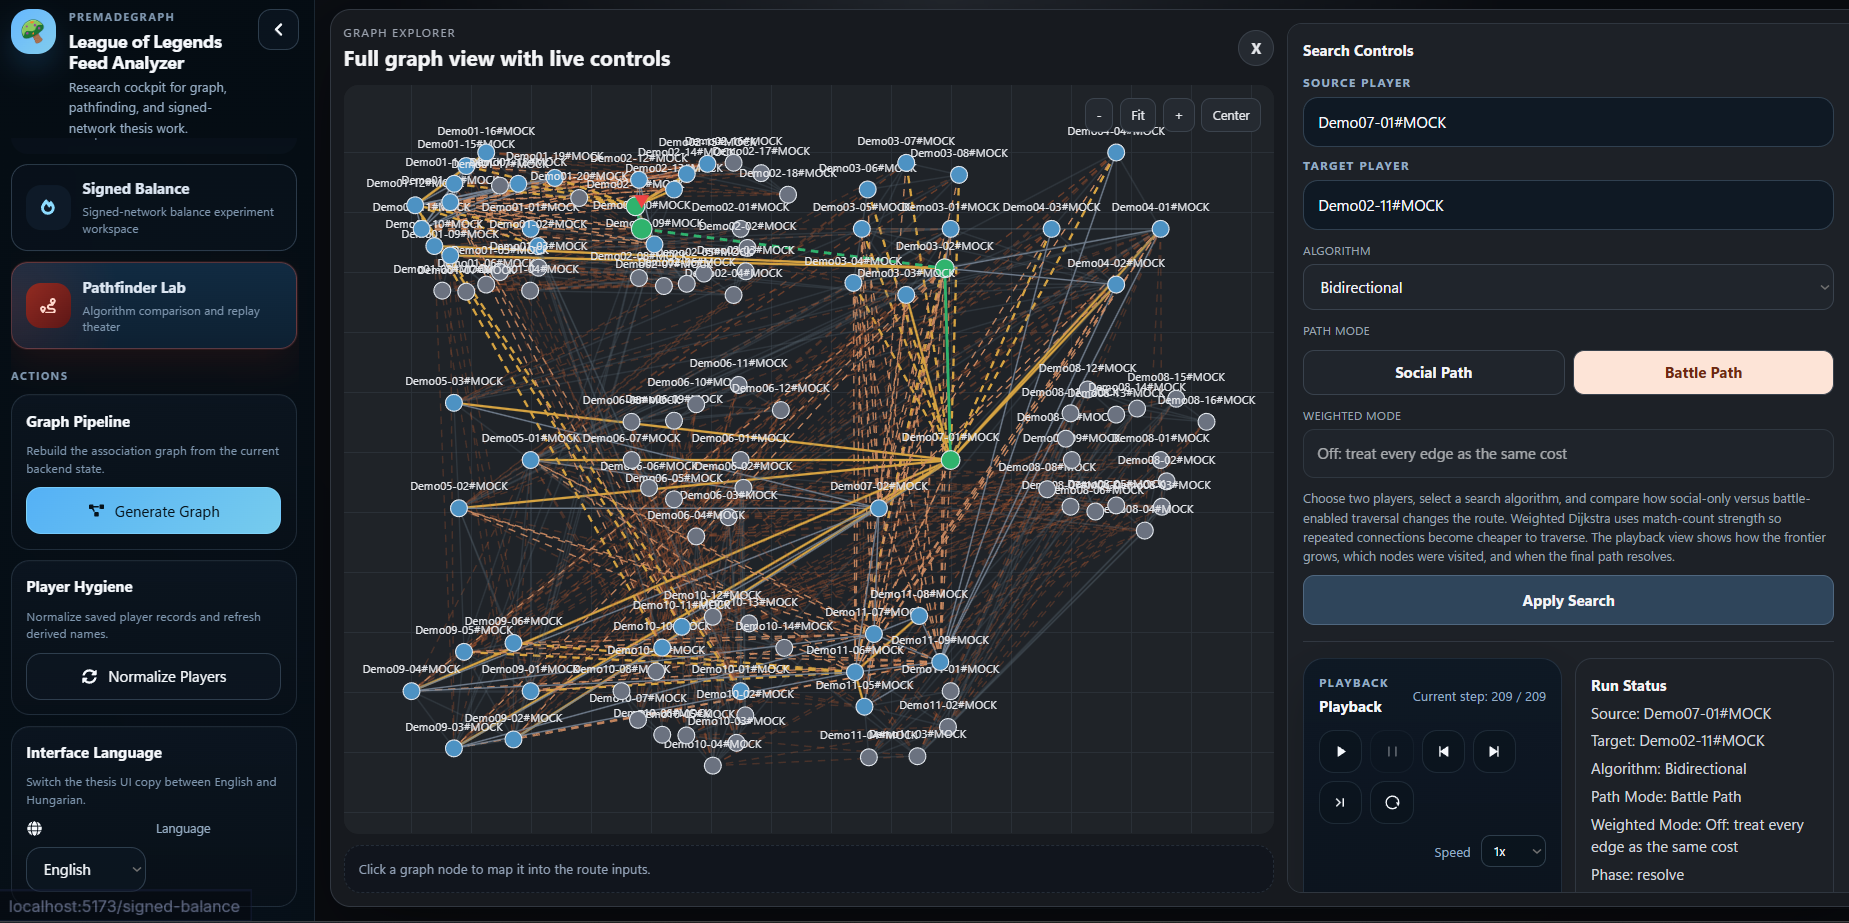
\includegraphics[width=0.9\textwidth]{mock-test-pathfinder-end.png}
    \caption{Összehasonlító állapot a Pathfinder Lab egyik tesztjellegű futtatásából}
\end{figure}

\section{Miért fontos ez túl a UI-n?}

A Pathfinder Lab azért kap külön fejezetet, mert valójában nem frontend-extra. Ez az a réteg, ahol a Rust algoritmusok, a backend-szerződések, a perzisztens játékosprofilok és a böngészőben értelmezhető interakció egyetlen működő demonstrációvá állnak össze. Ha a dolgozat célja az, hogy az egész rendszer védhető legyen, akkor ezt a fejezetet nem lehet a vizuális melléklet szintjére leszorítani.

\chapter{A 3D bird's-eye sphere és globális hálózati vizualizáció}

\section{A frontend szerepe}

A frontend jelenleg már nem egyetlen gráfnézet, hanem több, világosan elkülönített felületből álló mini-rendszer. Ez fontos minőségi ugrás a korábbi állapothoz képest, mert a projekt ekkor vált valóban bemutatható és narratívába rendezhető alkalmazássá.

A fő felületek:

\begin{itemize}
    \item \textbf{Match Analysis}: adatgyűjtési és mérkőzésellenőrző nézet,
    \item \textbf{Pathfinder Lab}: útvonalkeresési és algoritmus-összehasonlító nézet,
    \item \textbf{Full 3D Graph Sphere}: teljes hálózati madártávlat,
    \item \textbf{Signed Balance}: előjeles strukturális egyensúly-elemző oldal,
    \item \textbf{Assortativity}: teljesítmény-hasonlóságot vizsgáló analitikai oldal.
\end{itemize}

\section{Miért nem egyetlen képernyő?}

A felület több oldalra bontása nem esztétikai döntés volt, hanem használhatósági és védhetőségi kérdés. Egy szakdolgozati demo során sokkal könnyebb végigvezetni a nézőt azon az úton, hogy:

\begin{enumerate}
    \item adatot gyűjtünk vagy ellenőrzünk,
    \item gráfot és klasztereket generálunk,
    \item útvonalakat keresünk,
    \item globális struktúrát nézünk,
    \item kutatási jellegű elemzést futtatunk.
\end{enumerate}

Ha minden ugyanarra a képernyőre kerülne, a projekt inkább eszköztárnak, mintsem koherens rendszernek hatna.

\section{A 3D globális nézet}

A \emph{bird's-eye sphere} oldal a teljes hálózat vizuális áttekintésére szolgál. A legfontosabb tervezési döntés itt az volt, hogy a böngésző ne valós időben számolja a teljes layoutot, hanem a Rust réteg előre exportáljon minden fontos artifaktumot, és a frontend csak rendereljen.

Ennek több előnye van:

\begin{itemize}
    \item a layout determinisztikusabb,
    \item a demók megismételhetők,
    \item a böngésző terhelése kisebb,
    \item a vizuális réteg jobban elválik a számítási rétegtől.
\end{itemize}

\section{A bird's-eye manifest technikai tartalma}

A 3D nézethez tartozó előre generált manifest a dolgozat írásakor a következő nagyságrendi képet mutatta:

\begin{itemize}
    \item \textbf{25\,438} csúcs,
    \item \textbf{145\,959} él,
    \item \textbf{60\,997} ally-jellegű él,
    \item \textbf{84\,962} enemy-jellegű él,
    \item \textbf{24\,106} klasztercsoport,
    \item \textbf{420.0} sugarú gömbi elrendezés,
    \item körülbelül \textbf{17\,949 ms} generálási idő.
\end{itemize}

Ezek a számok két dolgot tesznek láthatóvá. Egyrészt a vizualizáció nem néhány száz csúcsos demóra épül, hanem valóban nagyméretű gráfra. Másrészt a 3D nézet mögött ugyanúgy mérhető, exportált futás áll, mint a kutatási analitikák mögött.

A \texttt{server.js} és a bird's-eye exportútvonalak alapján a 3D nézet mögött több, külön felelősségű artifaktum áll. A frontend nem egyetlen nagy JSON-fájlt tölt be, hanem manifesztet és bináris tömböket fogyaszt.

\begin{table}[H]
\centering
\caption{A bird's-eye export fő artifaktumai}
\begin{tabularx}{\textwidth}{>{\raggedright\arraybackslash}p{4.2cm}X}
\toprule
\textbf{Fájl} & \textbf{Szerep} \\
\midrule
\texttt{manifest.json} & Metaadatok, darabszámok, skálázási és generálási információk \\
\texttt{node\_meta.json} & Csomópontszintű leíró metaadatok, frontend-hozzárendelések \\
\texttt{node\_positions.f32} & Lebegőpontos koordináták tömbje a gyors rendereléshez \\
\texttt{node\_metrics.u32} & Tömörített numerikus csomóponti mutatók \\
\texttt{edge\_pairs.u32} & Él-végpontpárok tömbje \\
\texttt{edge\_props.u32} & Élhez tartozó kódolt tulajdonságok \\
\bottomrule
\end{tabularx}
\end{table}

Ez a bontás rendszerszinten jól indokolható. A nagy tömegű numerikus adat bináris marad, ami gyorsabb böngészőoldali feldolgozást tesz lehetővé, miközben az emberileg olvasható metaadat külön JSON-rétegben marad. A frontend tehát megjelenít, nem pedig újraszámol.

\begin{figure}[H]
    \centering
    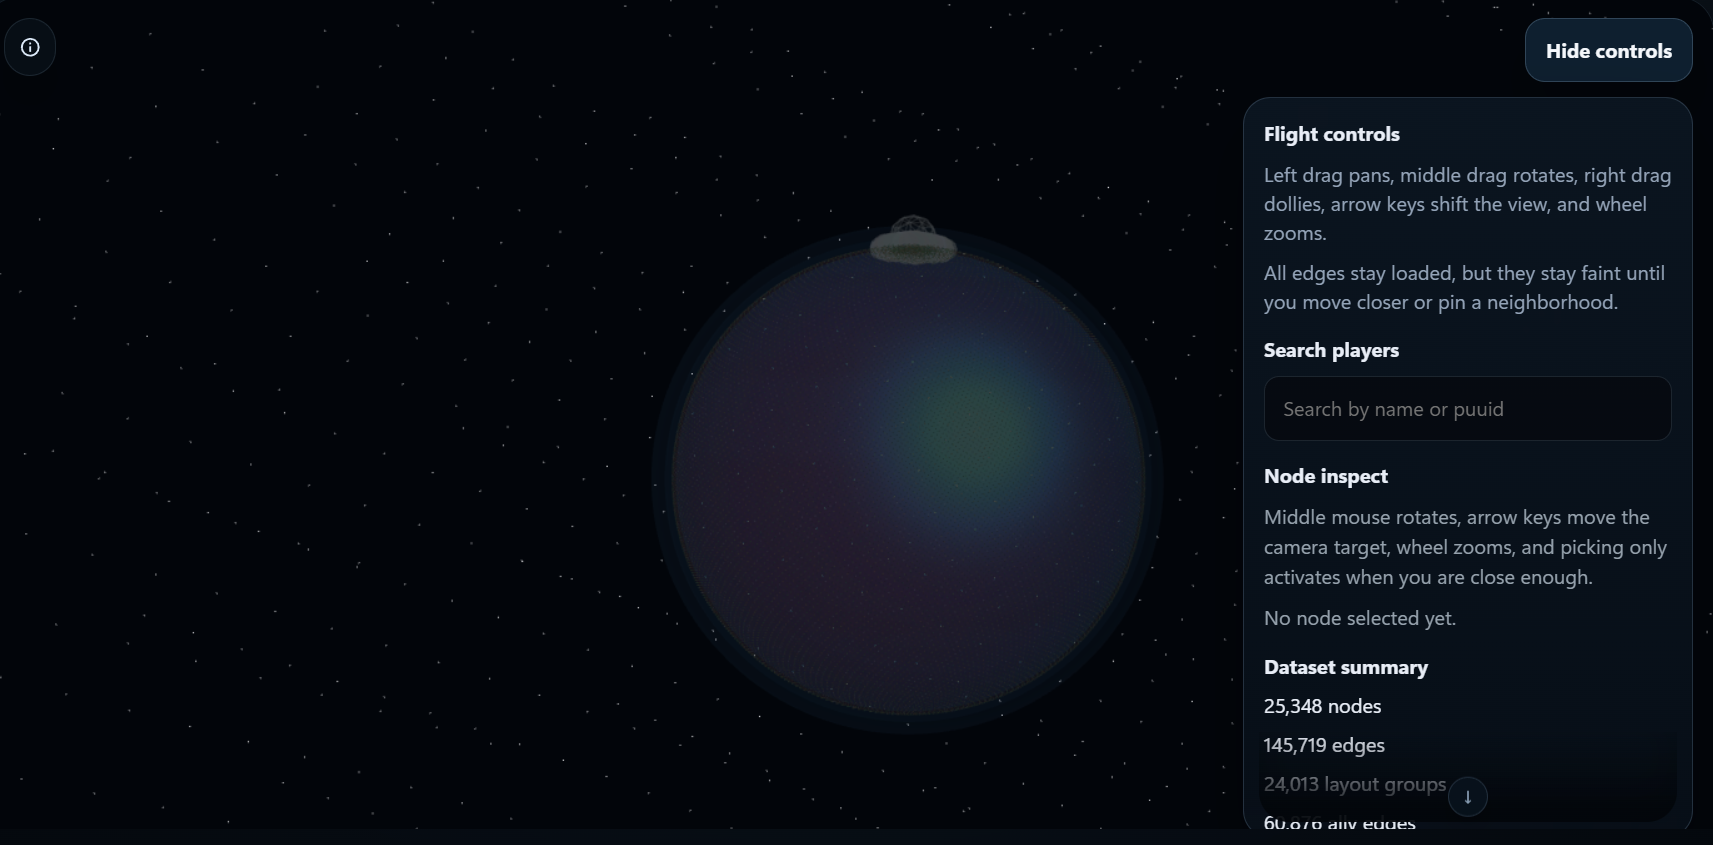
\includegraphics[width=0.92\textwidth]{birds-eye-current-state.png}
    \caption{A teljes hálózat 3D madártávlati nézete az előre generált Rust-artifaktumokra építve}
\end{figure}

\begin{figure}[H]
    \centering
    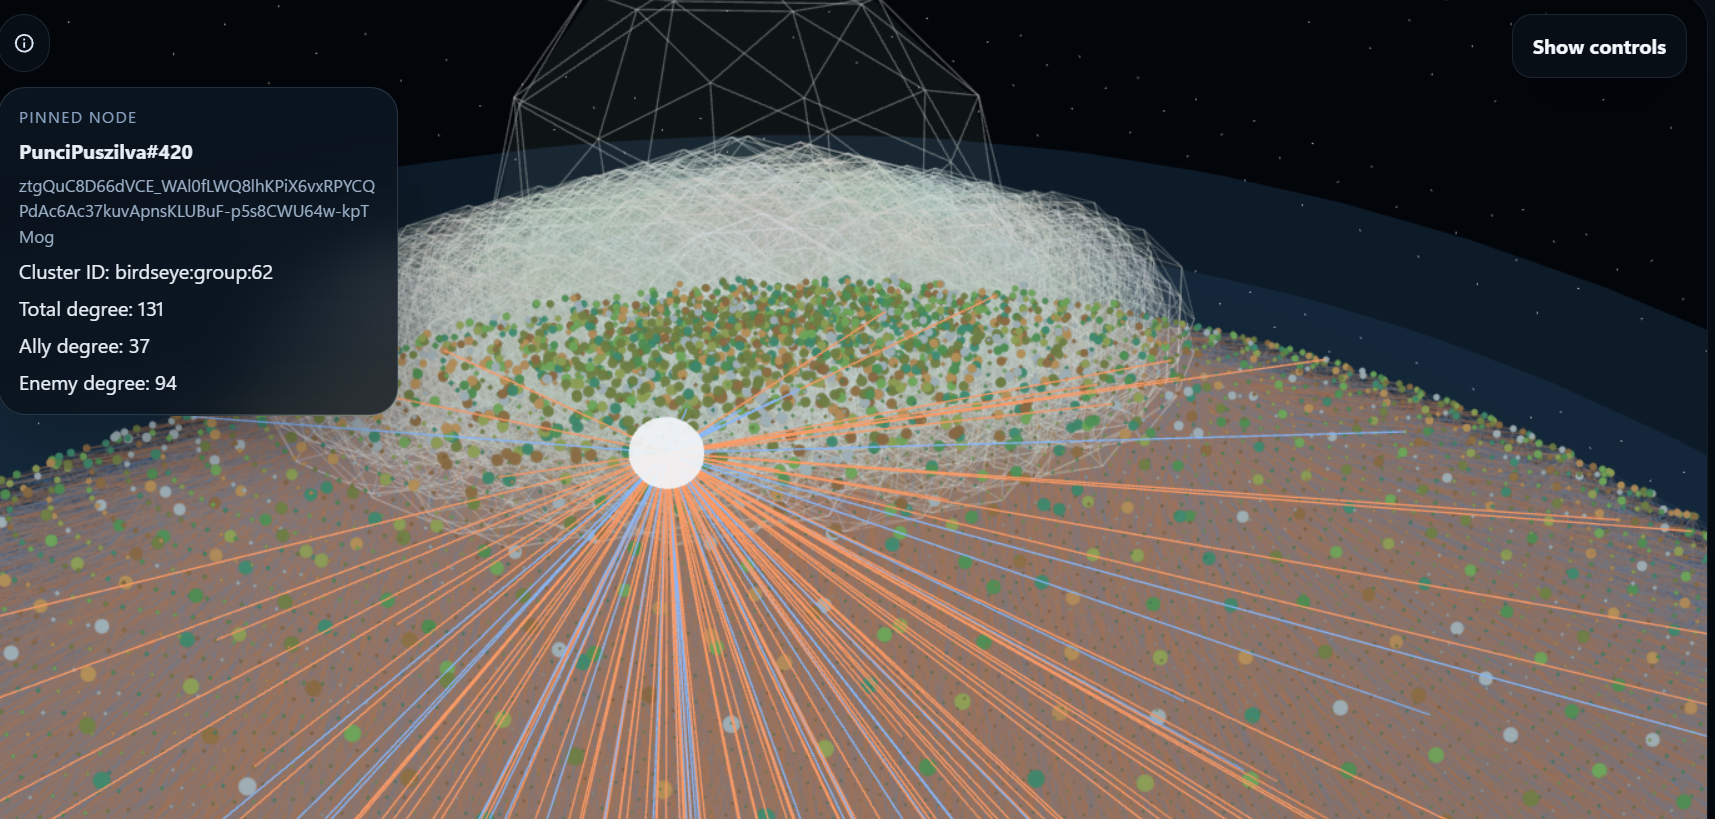
\includegraphics[width=0.82\textwidth]{birds-eye-cluster-view.png}
    \caption{Sűrűbb klaszterfoltok és a térbeli elkülönítés a globális nézetben}
\end{figure}

\begin{figure}[H]
    \centering
    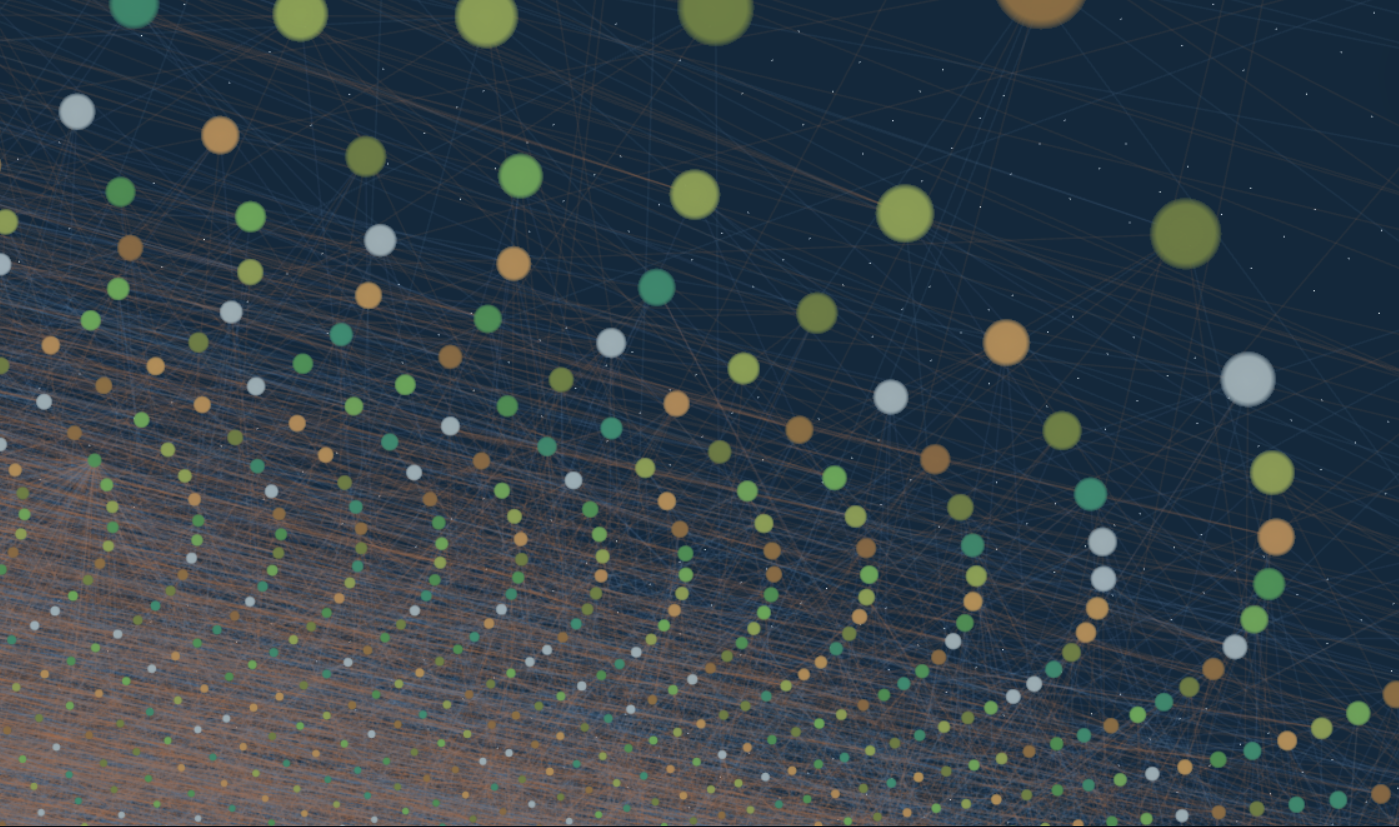
\includegraphics[width=0.78\textwidth]{birds-eye-individiual-web.png}
    \caption{Lokálisabb hálózati részlet a bird's-eye nézeten belül}
\end{figure}

\section{Pathfinder Lab}

A Pathfinder Lab az a felület, ahol a gráf nem elsősorban látványelemként, hanem algoritmikus térként jelenik meg. A felület támogatja:

\begin{itemize}
    \item forrás- és céljátékos kiválasztását,
    \item több algoritmus összehasonlítását,
    \item visszajátszási és léptetési funkciókat,
    \item súlyozott és nem súlyozott módot,
    \item többféle útvonalmód közötti váltást.
\end{itemize}

\begin{figure}[H]
    \centering
    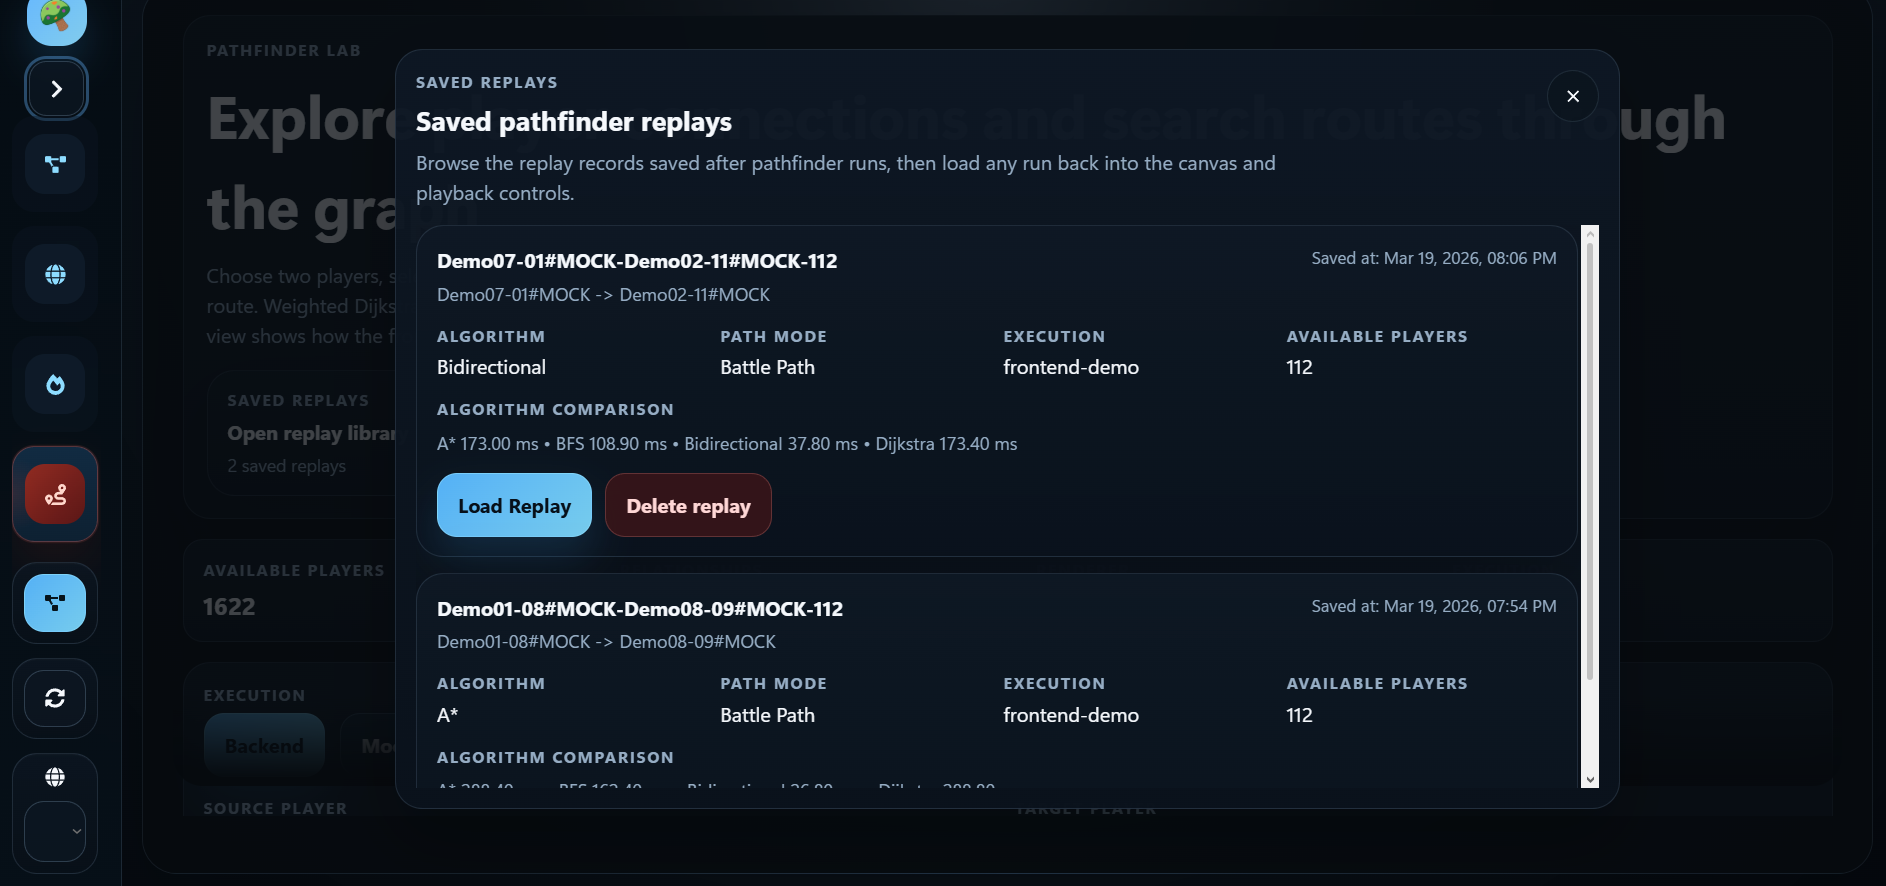
\includegraphics[width=0.92\textwidth]{pathfinder-replay-panel.png}
    \caption{Útvonalkeresési és visszajátszási felület a Pathfinder Lab oldalon}
\end{figure}

\section{Signed Balance és Assortativity oldalak}

A két kutatás-orientált oldal közös tulajdonsága, hogy nem elégednek meg egyetlen backend-válasz megjelenítésével. Mindkettő igyekszik:

\begin{itemize}
    \item magyarázni a kontrollok jelentését,
    \item megmutatni a pipeline-összefüggéseket,
    \item elkerülni a túl gyors, túl erős társadalmi következtetéseket.
\end{itemize}

Ez különösen fontos, mert az ilyen típusú analitika könnyen félreértelmezhető. A felület ezért szándékosan tartalmaz interpretációs szövegeket és magyarázó elemeket is.

\begin{figure}[H]
    \centering
    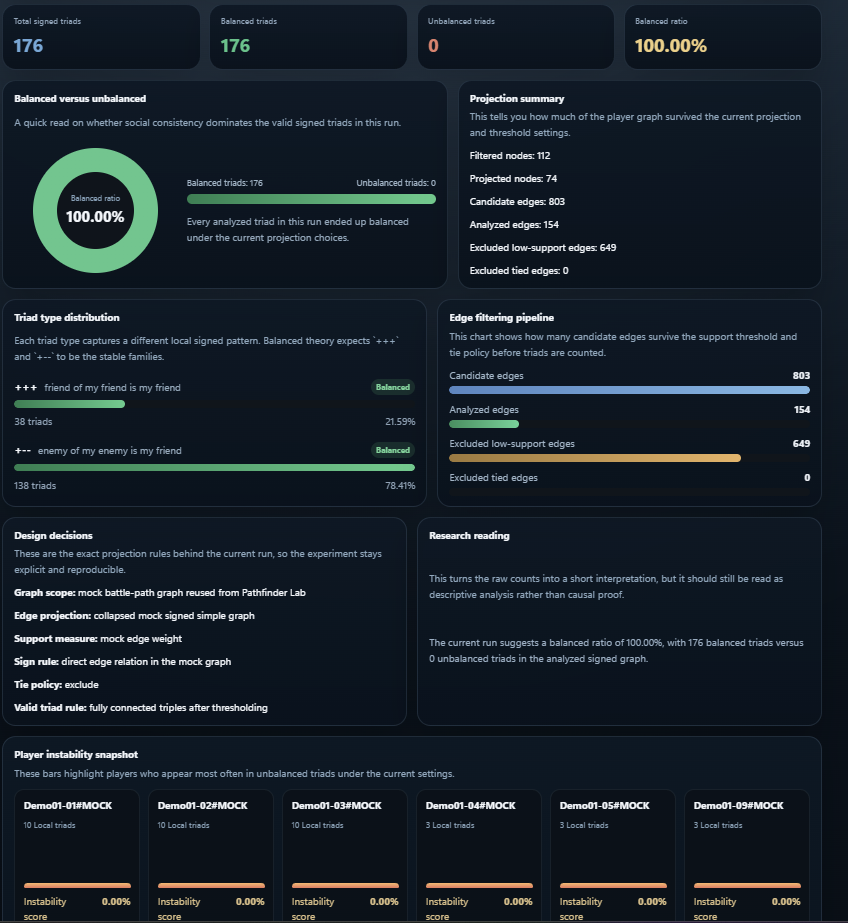
\includegraphics[width=0.92\textwidth]{sign-page.png}
    \caption{A strukturális egyensúly-elemző oldal a jelenlegi frontendben}
\end{figure}

\section{Diagramok és belső fejlesztői dokumentáció}

A repository dokumentációs csomagja több vektorgrafikus rendszerábrát is tartalmaz (\texttt{activity diagram.pdf}, \texttt{system statemachine research pipeline.pdf}, \texttt{uml simplified vector\_2.pdf}). Ezekből nem mindegyik került végleges, beégetett képként a dolgozat törzsébe, de fejlesztés közben fontos szerepük volt abban, hogy a rendszer ne essen szét egymásra rakódó feature-ök halmazára.

\diagramfigure{Állapotgép a kutatási pipeline fő lépéseihez}{system statemachine research pipeline.pdf}

\chapter{Előjeles gráfmodell és strukturális egyensúly}

\section{Miért természetes az előjeles modell ebben a projektben?}

A jelenlegi adatmodell egyik legérdekesebb következménye, hogy ugyanazon játékospár között nem csak ``kapcsolat van vagy nincs'', hanem a kapcsolat jellege is mérhető. A Rust gráfállapot külön tárolja az \texttt{allyWeight} és \texttt{enemyWeight} értékeket, vagyis azt, hogy két játékos hányszor szerepelt ugyanazon, illetve ellentétes oldalon. Ebből viszonylag természetes módon képezhető előjeles egyszerű gráf.

Ez a lépés azért fontos, mert a rendszer itt lép túl a hagyományos együtt-játszási hálón. Az él már nem pusztán ismétlődő kontaktus, hanem társas viszonytípus-projekció is.

\section{Az előjeles projekció döntései}

A jelenlegi implementáció a következő szabályokkal dolgozik:

\begin{itemize}
    \item ha az \texttt{allyWeight} dominál, az él pozitív;
    \item ha az \texttt{enemyWeight} dominál, az él negatív;
    \item ha a két érték döntetlen, akkor alapértelmezés szerint az él kiesik;
    \item az elemzés minimum támogatási küszöböt használ.
\end{itemize}

Formálisan a domináns előjel felírható a következő egyszerű szabállyal:

\begin{equation}
\operatorname{sign}(u,v)=
\begin{cases}
+1, & \text{ha } ally(u,v) > enemy(u,v) \\
-1, & \text{ha } enemy(u,v) > ally(u,v) \\
\text{nincs él}, & \text{ha } ally(u,v)=enemy(u,v)
\end{cases}
\end{equation}

Ez nem az egyetlen lehetséges projekció, de a jelenlegi rendszerben jól dokumentálható és determinisztikus kiindulópont.

A \texttt{signed\_balance.rs} modul ezt nem rejtett belső szabályként kezeli, hanem a kimenetben is dokumentálja: a vizsgált gráf a szűrt runtime-háló, a multi-edge előzmény egyszerű signed élre van összehúzva, a támogatás az \texttt{allyWeight + enemyWeight} összegből származik, a döntetlen él pedig alapértelmezésben kiesik. Ez módszertanilag kulcsfontosságú, mert a signed balance arány önmagában félrevezető lehetne a projekciós szabályok ismerete nélkül.

Fontos ugyanakkor kimondani a leegyszerűsítést is: két játékos kapcsolata a valóságban lehet vegyes történetű, vagyis sem nem tisztán „pozitív”, sem nem tisztán „negatív”. A jelenlegi modul nem folytonos bizonytalanságot modellez, hanem domináns viszonyt rögzít. Ez egyszerre erősség és korlát: nagyon jól auditálható, viszont bizonyos árnyalatokat szükségképpen elvesz.

\section{Triádok osztályozása}

A strukturális egyensúly háromcsúcsú, teljesen összekapcsolt részgráfokon értelmeződik. A klasszikus felosztás alapján a \texttt{+++} és a \texttt{+--} típus kiegyensúlyozott, míg a \texttt{++-} és a \texttt{---} típus kiegyensúlyozatlan. A jelenlegi modul ezt a logikát gépi úton enumerálja, majd nemcsak összesített arányt, hanem triádtípus-eloszlást és csomóponti részvételi mutatókat is visszaad.

Ez azért fontos, mert a kimenet így nem egyetlen ``balance ratio'' számra zsugorodik. A dolgozatban különösen értékes, hogy látható, mely játékosok vesznek részt a ritkább, instabil triádokban.

Algoritmikai oldalról a triádelemzés teljesen összekapcsolt hármasokra korlátozódik. A modul a szomszédsági metszetekből indul ki, vagyis nem az összes lehetséges háromcsúcsú kombinációt vizsgálja végig vakon, hanem csak azokat a jelölteket, ahol minden szükséges él ténylegesen jelen van és átmegy a support-szűrőn. Ez különösen fontos a védhetőség szempontjából: a rendszer nem feltételez hiányzó kapcsolatokat, hanem a megfigyelt signed maghálót elemzi.

\section{A tényleges futtatás eredménye}

A 2026. április 24-én ellenőrzött alapfuttatásnál a paraméterek a következők voltak:

\begin{itemize}
    \item minimális él-támogatás: 2,
    \item döntetlen-kezelés: kizárás,
    \item top instabil csúcsok listázása: bekapcsolva,
    \item klaszterösszegzés: bekapcsolva.
\end{itemize}

Az eredmény különösen erős kiegyensúlyozottságot mutatott: \textbf{3734} triádból \textbf{3732} bizonyult kiegyensúlyozottnak. Az instabil esetek száma mindössze \textbf{2} volt. A top instabil csúcsok között megjelent például az \texttt{EnRonin} nevű játékos, akinél a lokális instabilitási arány a kevés, de valós példában már látható volt.

Ez a nagyon magas arány azonban csak a teljes szűrési kontextussal együtt értelmezhető. A jelölt élek száma nagyságrendekkel magasabb volt, mint a végül elemzett éleké, vagyis a signed analízis egy erősen megszűrt hálómagon futott. Ez nem gyengeség, hanem a módszer következetessége: a modul inkább kizár bizonytalan kapcsolatokat, minthogy gyenge bizonyítékból kényszerítsen előjelet. Emiatt a balance-ratio egyik implicit jelentése az is, hogy a stabilabb, domináns viszonyokból álló magháló rendkívül rendezett szerkezetet mutat.

\section{Érzékenységvizsgálat: mi történik, ha a projekciót megpiszkáljuk?}

A rendszer egyik legerősebb kutatási eleme, hogy a signed-balance nem áll meg egyetlen futásnál. A \texttt{balance-sweep} runner több küszöb- és tie-policy kombinációt is képes lefuttatni. A vizsgált sweep összefoglalása:

\begin{table}[H]
\centering
\caption{Signed-balance érzékenységvizsgálat kiválasztott futásai}
\begin{tabular}{lrrr}
\toprule
\textbf{Min. support} & \textbf{Tie policy} & \textbf{Triádok száma} & \textbf{Balanced ratio} \\
\midrule
1 & exclude & 405\,921 & 0.99916 \\
1 & ally & 405\,921 & 0.99469 \\
1 & enemy & 405\,921 & 0.99460 \\
2 & exclude & 3734 & 0.99946 \\
2 & ally & 3734 & 0.98311 \\
2 & enemy & 3734 & 0.97963 \\
3 & exclude & 1052 & 0.99905 \\
4 & exclude & 210 & 1.00000 \\
\bottomrule
\end{tabular}
\end{table}

Ez a táblázat szakdolgozati szempontból kulcsfontosságú. A legerősebb állítás ugyanis nem az, hogy ``a háló kiegyensúlyozott'', hanem az, hogy \emph{a jelenlegi korpuszban a strukturális egyensúlyra utaló jel erős, de az arány érzékeny a döntetlenek kezelésére}. Ez sokkal védhetőbb és őszintébb következtetés.

\section{Mit jelent ez a projekt egészére nézve?}

A signed-balance fejezet azért különösen értékes, mert megmutatja, hogy a projekt valóban átlépett a ``vizualizáljunk egy gráfot'' szintről a kutatási jellegű hálózatelemzés felé. A rendszer már nem csak arról szól, hogy ki kivel játszott, hanem arról is, hogy az ismétlődő interakciókból milyen lokális társas szerkezet olvasható ki.

\chapter{Asszortativitási elemzés}

\section{Az asszortativitás szerepe a dolgozatban}

Az asszortativitás azért lett külön kiemelt analitikai irány, mert egyszerre könnyen magyarázható és módszertanilag tiszta. A kérdés itt nem az, hogy ki ``jobb'' játékos, hanem az, hogy az összekapcsolt játékosok hajlamosak-e hasonló teljesítményprofilhoz tartozni.

A projektben ez különösen jó illeszkedés, mert a gráf és a játékosprofil már korábban is létezett. Nem kellett új, bizonytalan címkét bevezetni; elég volt a meglévő \texttt{opscore} és \texttt{feedscore} metrikákat a gráfél-végpontokra vetíteni.

\section{A számítási definíció}

A jelenlegi implementáció numerikus asszortativitást számol Pearson-korreláció formájában. Ha az él egyik végpontján mért értékeket $x_i$, a másik végpontén mért értékeket pedig $y_i$ jelöli, akkor az együttható a szokásos formában írható fel:

\begin{equation}
r = \frac{\sum_i (x_i-\bar{x})(y_i-\bar{y})}{\sqrt{\sum_i (x_i-\bar{x})^2}\sqrt{\sum_i (y_i-\bar{y})^2}}
\end{equation}

A projekt ezt két fontos kiterjesztéssel használja:

\begin{itemize}
    \item külön kezeli a \texttt{social-path} és \texttt{battle-path} gráfmódot;
    \item a globális együttható mellett külön bontásokat is képez klaszteren belüli, klaszterek közötti, illetve erős és gyenge kapcsolatok szerint.
\end{itemize}

A \texttt{backend/pathfinder-rust/src/engine/assortativity.rs} egyik lényeges technikai döntése, hogy az irányítatlan éleket mindkét endpoint-orientációval figyelembe veszi a Pearson-akkumulációban. Ez azért védhető, mert az élnek nincs természetes iránya, ugyanakkor a két végpont tulajdonságpárja szimmetrikusan járul hozzá a korrelációhoz. A modul emellett külön számlálja az alacsony támogatás, a hiányzó score és a túl rövid játékostörténet miatt kihagyott éleket is. Így az asszortativitási eredmény nem egy feketedoboz-korreláció, hanem egy jól dokumentált mintaképzési folyamat eredménye.

\section{A fő eredmények részletesebb bontásban}

A központi futtatás négy headline eredménye már korábban is megjelent, de a részletes kimenet ennél sokkal gazdagabb volt. A következő táblázat a főbb bontásokat foglalja össze:

\begin{table}[H]
\centering
\caption{Részletes asszortativitási bontások az aktív dataseten}
\begin{tabular}{llrr}
\toprule
\textbf{Gráfmód} & \textbf{Bontás} & \textbf{opscore} & \textbf{feedscore} \\
\midrule
\texttt{social-path} & globális & 0.4744 & 0.3268 \\
\texttt{social-path} & klaszteren belül & 0.2888 & 0.2164 \\
\texttt{social-path} & klaszterek között & 0.4790 & 0.3296 \\
\texttt{social-path} & erős kapcsolatok & 0.2332 & 0.2230 \\
\texttt{social-path} & gyenge kapcsolatok & 0.4756 & 0.3275 \\
\texttt{battle-path} & globális & 0.4183 & 0.0101 \\
\texttt{battle-path} & klaszteren belül & 0.2665 & 0.1405 \\
\texttt{battle-path} & klaszterek között & 0.4204 & 0.0082 \\
\texttt{battle-path} & erős kapcsolatok & 0.2353 & 0.2022 \\
\texttt{battle-path} & gyenge kapcsolatok & 0.4187 & 0.0094 \\
\bottomrule
\end{tabular}
\end{table}

\section{Mit mondanak ezek a számok?}

Két jelenség különösen érdekes.

Elsőként az \texttt{opscore} minden vizsgált módon pozitív asszortativitást mutat. Ez arra utal, hogy a kapcsolódó játékosok teljesítményprofilja ezen a kompozit metrikán nem keveredik teljesen véletlenszerűen. Nem állítom, hogy ez önmagában oksági magyarázat, de az biztosan látszik, hogy a gráf és a score-réteg között érdemi kapcsolat van.

Másodszor a \texttt{feedscore} viselkedése jóval érzékenyebb a gráf definíciójára. A \texttt{social-path} módban még mérsékelt pozitív jel látható, míg a \texttt{battle-path} globális értéke gyakorlatilag nullához közeli. Ez azt sugallja, hogy a negatív vagy ellenfél-jellegű interakciók bevonásával a hasonlósági szerkezet jelentősen megváltozik.

Ez a különbség a projekt egyik legérdekesebb eredménye. Ha minden metrika minden gráfmódban hasonlóan viselkedne, akkor könnyen lehetne azt mondani, hogy a gráfdefiníció csak technikai csomagolás. A jelen esetben azonban a \texttt{feedscore} szinte nullára esik a \texttt{battle-path} módban, miközben a \texttt{social-path} hálón még látható együttmozgás marad. Ez arra utal, hogy a kapcsolatok szemantikája ténylegesen befolyásolja a teljesítményhasonlóság szerkezetét.

\section{A randomizációs infrastruktúra helye}

A kódbázisban az asszortativitáshoz randomizációs szignifikanciateszt is tartozik. Ez fontos fejlesztési irány, mert a leíró korrelációt nullmodellel is érdemes összevetni. A jelen dolgozatban azonban a fő eredményeket a közvetlenül ellenőrzött leíró és bontott futtatásokra alapozom. Így a szöveg őszinte marad: a szignifikanciakeret jelen van a rendszerben, de a hangsúly még nem a teljes permutációs kísérletsorozaton van.

\begin{figure}[H]
    \centering
    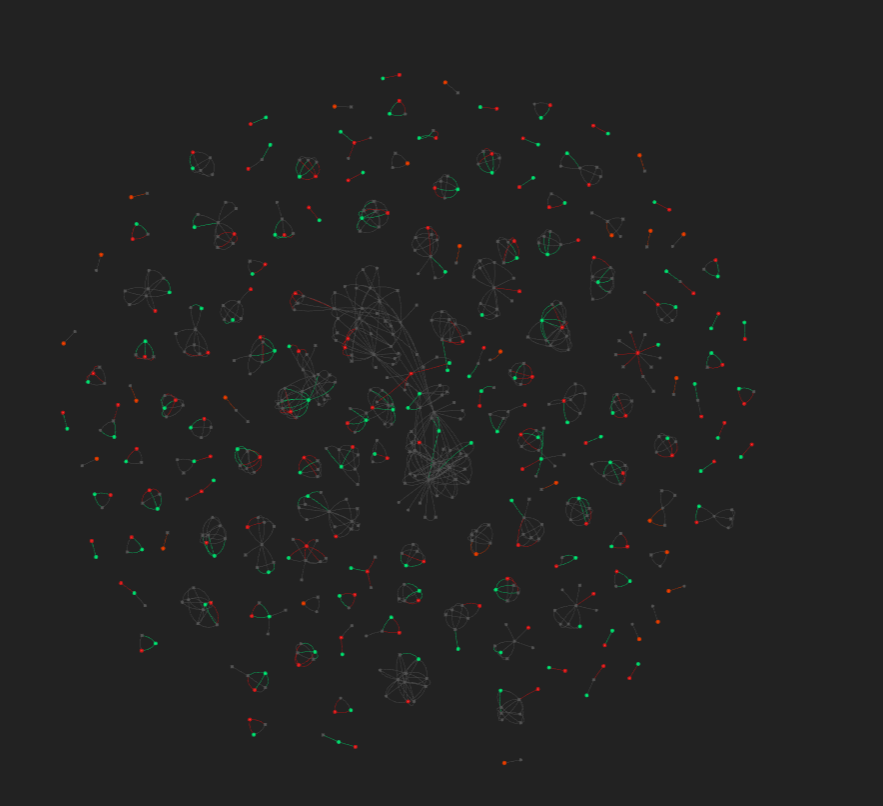
\includegraphics[width=0.9\textwidth]{associative-graph.png}
    \caption{Az asszortativitási oldal vizuális összefoglalója a jelenlegi frontendben}
\end{figure}

\chapter{Kísérleti futtatások, validáció és eredmények}

\section{Verifikációs lépések}

A dolgozat elkészítésekor a rendszer aktuális állapotát nemcsak a dokumentáció, hanem közvetlen futtatás alapján is ellenőriztem. A főbb helyi ellenőrzések:

\begin{itemize}
    \item a Rust futtatókörnyezet sikeresen lefuttatta az \texttt{assortativity} parancsot;
    \item a Rust futtatókörnyezet sikeresen lefuttatta a \texttt{signed-balance} parancsot;
    \item a fő adatbázis és dataset-nyilvántartás elérhető és olvasható volt;
    \item a frontendhez tartozó oldalak és típusdefiníciók fizikailag is jelen vannak a repositoryban.
\end{itemize}

Ez azért lényeges, mert a dolgozat ezen a ponton már nem csak tervekről, hanem ténylegesen végrehajtható modulokról számol be.

A verifikációs lépések tudatosan nem teljes funkcionalitástesztek voltak, hanem tézisszintű ellenőrzések. A cél itt az volt, hogy minden olyan rétegről legyen közvetlen bizonyíték, amelyre a dolgozat állításokat épít: a dataset-regiszter olvashatósága, a Rust analitikai parancsok futtathatósága, valamint a frontendoldalak fizikai jelenléte. Ez összhangban van a reprodukálható kutatási gyakorlat logikájával is: a szöveg és az alátámasztó futások között legyen világos kapcsolat \cite{sandve2013}.

\section{Az aktív állapot összefoglalása}

A 2026. április 24-én ellenőrzött aktív állapotban a rendszer a \texttt{default} datasetre épült. Az adatkészlet és a gráfállapot rövid összefoglalása:

\begin{table}[H]
\centering
\caption{A jelenlegi rendszerállapot fő mennyiségi mutatói}
\begin{tabular}{lr}
\toprule
\textbf{Mutató} & \textbf{Érték} \\
\midrule
Meccs-JSON állományok száma az aktív datasetben & 3471 \\
Játékosok száma a finomított adatbázisban & 25\,618 \\
\texttt{python\_population} klaszterek száma & 271 \\
\texttt{rust\_pathfinding} klaszterek száma & 269 \\
\texttt{cluster\_members} rekordok száma & 3227 \\
Signed-balance projektált csomópontok száma & 1527 \\
Signed-balance analizált élek száma & 3013 \\
\bottomrule
\end{tabular}
\end{table}

Ezeket a számokat nem szabad egyetlen homogén sokaságként olvasni. A \texttt{25\,618} játékos a teljes score-réteg kiterjedését mutatja, míg a signed balance számára releváns \texttt{1527} csomópont már egy erősen megszűrt részgráfhoz tartozik. Hasonlóképpen a \texttt{3471} meccsállomány a nyers korpusz nagysága, míg a klasztertagsági rekordok csak azon csúcsokhoz kötődnek, amelyek a perzisztált közösségi nézetekben is megjelennek. A dolgozat eredményei ezért lépcsőzetes mintákon állnak: minden réteg a saját, előzőekből leszűkített univerzumán számol.

\section{A korpusz összetétele mint értelmezési háttér}

Az eredmények értékeléséhez fontos hozzárakni, hogy a vizsgált korpusz nem homogén. A queue-eloszlás alapján a ranked módok dominálnak, de a rendszerben ARAM és normál meccsek is jelen vannak. Ez két következménnyel jár:

\begin{itemize}
    \item a gráf egy része erősen kompetitív, ismétlődő társas térből származik;
    \item egy másik része lazább, zajosabb kapcsolatokkal terhelt.
\end{itemize}

Éppen ezért a küszöbölés, az erős és gyenge kapcsolatok bontása, valamint a \texttt{social-path} és \texttt{battle-path} megkülönböztetése nem puszta technikai részlet, hanem az adatkorpuszból fakadó szükségszerűség.

Ez a felismerés a teljes eredményfejezetet meghatározza. Ha a korpusz heterogén, akkor a gráfmodellt sem lehet úgy kezelni, mintha egyetlen társas mechanizmust mérne. A \texttt{social-path} és \texttt{battle-path} különválasztása nem csupán algoritmus-beállítás, hanem módszertani védekezés a túlzó interpretáció ellen.

\section{A két klasztercsalád gyakorlati különbsége}

A perzisztált klasztereknél az is ellenőrizhető volt, hogy a Python és a Rust család eltérő karakterű. A \texttt{python\_population} klaszterek kicsit kisebb maximális méretűek és inkább populációs közösségképet adnak, míg a \texttt{rust\_pathfinding} klaszterek futásidejű szempontokhoz igazodnak, és jóval nagyobb maximumklasztert is tartalmaznak.

Ez összhangban van a rendszertervvel. A két klasztercsalád nem egymás hibás duplikátuma, hanem eltérő feladatokra optimalizált nézet.

\section{Strukturális egyensúly eredményei}

A \texttt{signed-balance} modul alapértelmezett futtatásának eredménye a következő volt:

\begin{table}[H]
\centering
\caption{A strukturális egyensúly futtatás fő eredményei}
\begin{tabular}{lr}
\toprule
\textbf{Mutató} & \textbf{Érték} \\
\midrule
Minimális él-támogatás & 2 \\
Döntetlen-kezelés & kizárás \\
Jelölt élek száma & 147\,265 \\
Analizált élek száma & 3013 \\
Alacsony támogatás miatt kizárt élek & 143\,965 \\
Döntetlen miatt kizárt élek & 287 \\
Analizált triádok száma & 3734 \\
Kiegyensúlyozott triádok száma & 3732 \\
Kiegyensúlyozatlan triádok száma & 2 \\
Kiegyensúlyozottsági arány & 0.99946 \\
\bottomrule
\end{tabular}
\end{table}

A triádtípusok bontása:

\begin{table}[H]
\centering
\caption{Triádtípusok eloszlása a jelenlegi projekció mellett}
\begin{tabular}{lrr}
\toprule
\textbf{Triádtípus} & \textbf{Kiegyensúlyozott?} & \textbf{Darabszám} \\
\midrule
\texttt{+++} & igen & 2153 \\
\texttt{++-} & nem & 1 \\
\texttt{+--} & igen & 1579 \\
\texttt{---} & nem & 1 \\
\bottomrule
\end{tabular}
\end{table}

Az eredmény első látásra rendkívül erős: a jelenlegi projekciós szabályok mellett a gráf szinte teljesen kiegyensúlyozott. Éppen ezért ezt az eredményt csak óvatosan lehet értelmezni. A védhető megfogalmazás nem az, hogy „a játékosközösség harmonikus”, hanem az, hogy:

\begin{quote}
a jelenlegi, domináns előjelre és legalább két kapcsolatra szűrt projekció mellett a megfigyelt teljesen összekapcsolt triádok döntő többsége strukturálisan kiegyensúlyozott.
\end{quote}

Ez a különbség nem retorikai finomkodás, hanem módszertani szükségszerűség. A magas arány ugyanis valószínűleg részben a küszöbölésből és a döntetlen-kizárásból is következik. Ugyanakkor ettől az eredmény még érdekes: azt mutatja, hogy a rendszer ténylegesen képes előjeles gráfot projektálni, triádokat enumerálni, és érdemi, nem triviális kimenetet előállítani.

Érdemes ezt a gyakorlat szintjén is pontosan megfogalmazni. A magas balance-ratio \emph{nem} azt jelenti, hogy a játékosközösség „harmonikus”, és azt sem, hogy társas értelemben stabil csoportokba szerveződik. A rendszer valójában ismétlődő mérkőzéskapcsolatokból számol domináns előjelet. A signed balance tehát sokkal inkább a projekciós szabályok és a stabil kapcsolati mag kombinált viselkedését méri, mintsem közvetlen pszichológiai vagy szociológiai valóságot. Ettől az eredmény nem értéktelenebb, csak szűkebben és pontosabban értelmezhető.

\section{Asszortativitási eredmények}

Ugyanezen a napon a Rust futtatókörnyezet \texttt{assortativity} parancsa a következő eredményeket adta:

\begin{table}[H]
\centering
\caption{A jelenlegi asszortativitási eredmények az aktív dataseten}
\begin{tabular}{llrr}
\toprule
\textbf{Gráfmód} & \textbf{Metrika} & \textbf{Korreláció} & \textbf{Mintaszám} \\
\midrule
\texttt{social-path} & \texttt{opscore} & 0.4744 & 61\,513 \\
\texttt{social-path} & \texttt{feedscore} & 0.3268 & 61\,513 \\
\texttt{battle-path} & \texttt{opscore} & 0.4183 & 147\,265 \\
\texttt{battle-path} & \texttt{feedscore} & 0.0101 & 147\,265 \\
\bottomrule
\end{tabular}
\end{table}

Az eredményekből több következtetés is levonható.

\subsection{Az \texttt{opscore} pozitívan asszortatív}

Mind a \texttt{social-path}, mind a \texttt{battle-path} nézetben jól látható pozitív korreláció jelenik meg az \texttt{opscore} mentén. Ez arra utal, hogy a gráfban összekapcsolt játékosok teljesítményprofilja ezen a metrikán nem véletlenszerűen keveredik.

Az is fontos, hogy az \texttt{opscore} pozitív asszortativitása nem tűnik el akkor sem, amikor a gráf jóval bővebbé válik a \texttt{battle-path} módban. Ez azt sugallja, hogy a kompozit teljesítménymutató robusztusabb hálózati szerkezetet fog meg, mint a direkt hibamutatóként értelmezett \texttt{feedscore}. Másképp fogalmazva: az \texttt{opscore} és a gráf között olyan kapcsolat látszik, amely túléli a kapcsolatvilág szemantikai tágítását is.

\subsection{A \texttt{feedscore} erősen függ a gráfmódtól}

Az egyik legérdekesebb megfigyelés, hogy a \texttt{feedscore} még közepesen pozitív asszortativitást mutat az ally-alapú \texttt{social-path} gráfon, de szinte teljesen eltűnik ez a kapcsolat a \texttt{battle-path} módban. Ez szakmailag sokkal érdekesebb annál, mint ha minden mindenhol pozitív lenne, mert azt jelzi, hogy a gráf jelentése tényleg számít.

A legóvatosabb, de már informatív értelmezés az, hogy:

\begin{itemize}
    \item a szövetségesi kapcsolatok mentén a \texttt{feedscore} még mutat némi hasonlósági szerkezetet,
    \item de amint az ellenfélkapcsolatok is bekerülnek a vizsgálatba, ez a szerkezet lényegében feloldódik.
\end{itemize}

\subsection{Belső és külső klaszterkapcsolatok}

A részletes kimenet azt is megmutatta, hogy az asszortativitás nem azonos erősségű a klaszteren belüli és klaszterek közötti kapcsolatoknál. Bár a legerősebb jel nem mindenhol belül jelent meg, az eredmények azt mutatják, hogy a klaszterinformáció önmagában még nem magyarázza ki teljesen a teljesítmény-hasonlóság szerkezetét. Ez további elemzési lehetőséget nyit meg a jövőre nézve.

Ez megint fontos módszertani figyelmeztetés. A klaszter nem egyenlő a teljesítményhomogenitással. A közösségi szerkezet és a metrikai hasonlóság kapcsolatban van egymással, de nem redukálható teljesen egymásra. Ez megerősíti, hogy a klaszterezési és a score-analitikai réteg külön-külön is értelmezendő.

\section{A frontend és a rendszerkoherencia értékelése}

A projekt egyik fontos eredménye nem kizárólag a számszerű analitikában áll, hanem abban is, hogy a rendszer ma már koherens egészként működik. A jelenlegi állapotban:

\begin{itemize}
    \item az adatgyűjtés és dataset-kezelés külön rétegben történik;
    \item a pontszámítás explicit, ellenőrizhető képletekre épül;
    \item a gráfépítés és klaszterezés nem ad hoc frontend-logika;
    \item a futásidejű Rust réteg a gráfanalitikát külön kezeli;
    \item a frontend több specializált felületen, eltérő célok mentén mutatja meg az eredményeket.
\end{itemize}

Ez azért fontos, mert a dolgozat nem egyszerűen egy algoritmus vagy egy látványos oldal bemutatása, hanem annak dokumentálása, hogy ezek a részek együtt már egy kutatásképes rendszerként viselkednek.

A koherencia egyik kézzelfogható jele, hogy a frontend route-struktúrája és a backend végpontstruktúrája egymásra illeszkedik. A \texttt{frontend/src/App.tsx} külön oldalakat tart fenn a collectorhoz, a graph sphere-hez, a signed-balance-hoz, az assortativity-hez és a Pathfinder Labhoz, vagyis a felület nem egyetlen „mindent bele” dashboard. Ez segít abban, hogy a felhasználó mindig ugyanannak a rendszernek egy konkrét analitikai nézőpontját lássa.

\section{A korábbi ország-elemzési ág helye a jelenlegi rendszerben}

A korábbi \texttt{assign\_countries.py} és \texttt{conclude.py} ág továbbra is a projekt része. Ez megőrzi azt a lehetőséget, hogy a klaszterekből származó országcímkézést összekapcsoljuk aggregált teljesítményelemzéssel. Ugyanakkor a jelenlegi dolgozat fő tudományos súlypontja már nem ez, hanem a gráf mint kutatási objektum.

Védhetőnek azt tartom, ha ezt az ország-elemzési vonalat \emph{kiegészítő, exploratív} modulnak nevezzük:

\begin{itemize}
    \item implementált,
    \item hasznos lehet,
    \item de bizonytalansága nagyobb,
    \item ezért a dolgozat központi állításait nem erre építem.
\end{itemize}

\chapter{Rendszerszintű értékelés és megvitatás}

\section{Mi bizonyult a legerősebb rendszertervezési döntésnek?}

Az egész projektet visszanézve a legerősebb döntésnek azt tartom, hogy a különböző feladatokat nem próbáltam egyetlen univerzális technológiába kényszeríteni. Az \texttt{architecture-decision} szemlélet alapján ez úgy fogalmazható meg, hogy a rendszer nem eszközpreferencia, hanem minőségi attribútumok mentén fejlődött. A fontos attribútumok a következők voltak:

\begin{itemize}
    \item reprodukálhatóság,
    \item magyarázhatóság,
    \item perzisztencia,
    \item futási teljesítmény,
    \item demo- és védhetőségi koherencia.
\end{itemize}

Ezek közül ritkán lehet mindent ugyanazzal az eszközzel a legjobban kiszolgálni. A Python gyors iterációt és kényelmes adatfeldolgozást ad, a Rust teljesítményt és pontos gráfkontrollt, a Node/Express stabil integrációs felületet, a React pedig erős bemutathatóságot. A többnyelvűség tehát itt nem öncélú komplexitás, hanem funkcionális specializáció.

\section{A rendszer erősségei}

A jelenlegi állapot alapján a projekt legfontosabb erősségei:

\begin{itemize}
    \item a teljes adatút végigkövethető a Riot API-tól a frontendig;
    \item a játékosprofilok explicit, ellenőrizhető képleteken és mezőkön alapulnak;
    \item a gráfépítés és klaszterezés nem csak vizuális export, hanem perzisztens objektum;
    \item a Rust réteg valódi analitikai és futtatási értéket ad, nem csak ``gyorsabb átírás'';
    \item a signed-balance és asszortativitás már valódi kutatási kérdésekké emelik a rendszert.
\end{itemize}

\section{Fenyegetések a validitásra}

Egy védhető szakdolgozatban legalább ennyire fontos kimondani a korlátokat is. A jelen projekt legfontosabb validitási kockázatai:

\begin{itemize}
    \item a dataset nem reprezentálja a teljes játékospopulációt;
    \item a gyűjtés seed- és queue-függő;
    \item a \texttt{feedscore} és \texttt{opscore} interpretálható, de nem ``igazságmérő'';
    \item a signed-balance eredménye érzékeny a projekciós és küszöbölési döntésekre;
    \item a country-ág sokkal bizonytalanabb, mint a közvetlen gráf- és meccsanalitika.
\end{itemize}

Ezek a korlátok azonban nem rombolják le a dolgozatot. Inkább kijelölik azt a határt, amelyen belül az állítások védhetők. Ezért is volt fontos, hogy a megvalósult és a jövőbeli elemeket szigorúan külön kezeljem.

Érdemes a validitási kockázatokat rétegenként is szétbontani:

\begin{itemize}
    \item \textbf{Mintavételi validitás}: a seedválasztás, a premade-probe és a queue-orientáció együtt nem véletlen mintát adnak a teljes játékospopulációból.
    \item \textbf{Mérési validitás}: a \texttt{feedscore} és \texttt{opscore} értelmezhető, de konstrukciós döntésekre épülő metrikák; különösen az \texttt{opscore} tartalmaz kézi szerepkör-súlyozást.
    \item \textbf{Projekciós validitás}: a signed balance domináns előjel-szabálya, a support-küszöb és a tie-policy érdemben alakítja a végső triádkészletet.
    \item \textbf{Klasztervaliditás}: a közösségdetektálás eredménye függ a választott gráftól, a küszöböléstől és a modularitás felbontási korlátjától \cite{fortunato_barthelemy2007}.
    \item \textbf{Időbeli validitás}: a korpusz fokozatosan épülő archívum, ezért a teljes háló nem egyetlen szinkron időpillanat felvétele.
\end{itemize}

Ezek a fenyegetések azonban nem cáfolják a projektet. Inkább megmutatják, hogy meddig lehet erős állításokat tenni, és hol kell tudatosan visszafogni az interpretációt. A dolgozat védhetőségét végső soron éppen ez a rétegzett őszinteség erősíti.

\section{Miért értékes a projekt szakdolgozatként?}

Szakdolgozati szempontból a projekt értéke nem csak abban áll, hogy ``sok mindent tud''. A valódi érték az, hogy több informatikai terület kapcsolódik össze benne:

\begin{itemize}
    \item adatgyűjtés és API-használat,
    \item adatbázistervezés,
    \item hálózatkutatás,
    \item algoritmusok és teljesítmény,
    \item frontend és vizuális kommunikáció.
\end{itemize}

Ez a kombináció azért erős, mert minden réteg hozzájárul a végső állításhoz. Ha bármelyik hiányozna, a dolgozat jóval gyengébb lenne: pusztán frontendként látványos lenne, pusztán algoritmusként kontextustalan, pusztán adatelemzésként pedig bemutatási réteg nélkül maradna.

Ehhez hozzáadódik a reprodukálhatósági érték is. A rendszer fő eredményei nem kézzel összeollózott prezentációs pillanatképekből állnak, hanem olyan pipeline-okból, amelyek a nyers meccs-JSON-tól a normalizált játékosprofilon és a perzisztált klasztereken át a Rust-analitikáig követhetők. Ez különösen erős szakdolgozati tulajdonság: a bemutatott állításokhoz tartozik egy végrehajtható technikai út is.

\section{A megvalósult és a jövőbeli elemek szétválasztása}

A dolgozat egyik tudatos módszertani döntése az volt, hogy a jelenleg implementált és a még csak tervezett elemeket nem keverem össze. A jelenlegi, ténylegesen megvalósult mag a következő:

\begin{itemize}
    \item Riot API-ra épülő adatgyűjtés;
    \item \texttt{puuid}-alapú normalizálás;
    \item \texttt{feedscore}/\texttt{opscore} számítás;
    \item Python gráfépítés és közösségdetektálás;
    \item SQLite klaszterperzisztencia;
    \item Rust útvonalkeresés és 3D globális export;
    \item signed-balance és asszortativitás.
\end{itemize}

A még nem lezárt, de már világosan kijelölt irányok:

\begin{itemize}
    \item párhuzamos Brandes-központiság;
    \item időbeli stabilitási és volatilitási mutatók;
    \item kohézió versus teljesítmény vizsgálata;
    \item adatvezérelt \texttt{opscore}-kalibráció.
\end{itemize}

Ez a szétválasztás nem gyengíti, hanem erősíti a dolgozatot. A bírálat szempontjából sokkal védhetőbb egy olyan szöveg, amely pontosan kijelöli a rendszer jelenlegi határát, mint egy olyan, amely minden jó ötletet kész eredménynek próbál feltüntetni.

\chapter{Összegzés}

\section{A projekt összefoglalása}

A dolgozatban bemutatott rendszer mára egy egyszerű premade gráfötletből olyan összetett, de világosan tagolt projektté fejlődött, amely képes:

\begin{itemize}
    \item valódi League of Legends meccsadatokat begyűjteni és adatkészletek szerint kezelni;
    \item a játékosokat \texttt{puuid} alapon normalizálni és szerepkörérzékeny mutatókkal leírni;
    \item az ismétlődő együtt- és egymás ellen játszásokból súlyozott és előjeles gráfokat építeni;
    \item közösségszerkezetet tárolni és újrafelhasználni;
    \item a Rust futtatókörnyezetben útvonalakat, globális nézeteket és analitikákat számolni;
    \item ezeket a kimeneteket több különálló, de koherens frontend oldalon bemutatni.
\end{itemize}

A jelenlegi rendszerállapot alapján a dolgozat legfontosabb üzenete számomra az, hogy ez a projekt már nem csak ötletszinten érdekes. A signed balance és az asszortativitás azt mutatják, hogy a hálózatban ténylegesen megfogható, mérhető szerkezetek jelennek meg. Közben a teljes architektúra is azt támasztja alá, hogy a rendszer nem véletlenszerűen összehordott komponensekből áll, hanem egyre inkább tudatosan szétválasztott felelősségi körök szerint fejlődött.

Az is fontos tanulság, hogy a projekt legerősebb része nem egyetlen „nagy trükk”. Nem az a lényege, hogy van benne 3D nézet, vagy hogy Rustban fut néhány algoritmus, vagy hogy vannak klaszterek. A valódi érték abban van, hogy az adatgyűjtés, a pontszámítás, a gráfépítés, a perzisztencia, az útvonalkeresés és a kutatási analitika végre ugyanannak a rendszernek a része.

\section{A dolgozat védhető fő következtetései}

Az aktuális implementáció alapján a következő állítások tekinthetők védhetőnek:

\begin{itemize}
    \item A League of Legends ismétlődő mérkőzésadataiból értelmes, több rétegben elemezhető játékosháló építhető.
    \item A szerepkörérzékeny, percentilis-alapú \texttt{opscore}/\texttt{feedscore} pipeline kellően értelmezhető ahhoz, hogy gráfanalitikai bemenetként használjuk.
    \item A Python és Rust közötti munkamegosztás a jelenlegi projektméretben indokolt és szakmailag jól védhető.
    \item A jelenlegi aktív adatkészleten az \texttt{opscore} mindkét gráfmódban pozitív asszortativitást mutat.
    \item A jelenlegi signed-balance projekció mellett a megfigyelt triádok szinte teljesen kiegyensúlyozottak, de ezt küszöb- és projekciófüggő eredményként kell értelmezni.
\end{itemize}

\chapter{Jövőbeli fejlesztések}

\section{Jövőbeli fejlesztési irányok}

A projekt jelenlegi állapotában már elég erős ahhoz, hogy a további fejlesztéseknél ne újabb random feature-öket, hanem célzott, tudományosan indokolható bővítéseket keressünk. A következő, még nem teljesen megvalósított, de kifejezetten erős irányok:

\begin{itemize}
    \item \textbf{Párhuzamos Brandes-féle központiság}: a Rust réteg és a meglévő gráfmodell kifejezetten alkalmas arra, hogy a betweenness centrality soros, majd \texttt{rayon}-alapú párhuzamos változata is bekerüljön \cite{brandes2001}.
    \item \textbf{Időbeli stabilitás és volatilitás}: a jelenlegi pontozás még dataset-alapú, nem időfüggő. A meccsek sorrendjéből később játékosonként stabilitási mutatók is levezethetők.
    \item \textbf{Közösségi kohézió és teljesítmény}: ha a klaszterekhez kohéziós mutatókat rendelünk, vizsgálhatóvá válik, hogy a szorosabb közösségek eltérő teljesítménymintát mutatnak-e.
    \item \textbf{Adatvezérelt \texttt{opscore}-kalibráció}: a jelenlegi rendszer átlátható, de kézi súlyokon alapul. Később egy továbbra is interpretálható, adatvezérelt kalibráció erősítheti a módszertant.
    \item \textbf{Erősebb nullmodellek}: különösen a strukturális egyensúly és az asszortativitás esetében értékes lenne a jelenlegi randomizációs infrastruktúrát tovább erősíteni.
\end{itemize}

\section{Zárszó}

Ha a projektet egy mondatban kellene összefoglalnom, azt mondanám: a \emph{Premade Graph} nem egyszerűen játékosstatisztikák megjelenítése, hanem egy olyan próbálkozás, amely a kompetitív játékot kapcsolati és analitikai térként kezeli. Ez a szemlélet tette lehetővé, hogy a meccsekből gráf, a gráfból közösség, a közösségből előjeles szerkezet, az előjeles szerkezetből pedig ténylegesen vitatható és megvédhető kutatási kérdés legyen.

\begin{thebibliography}{99}

\bibitem{riotportal}
\href{https://developer.riotgames.com/docs/portal}{Riot Developer Portal Documentation.}

\bibitem{riotapi}
\href{https://developer.riotgames.com/docs/lol}{Riot Games API Documentation for League of Legends.}

\bibitem{sqlite}
\href{https://www.sqlite.org/docs.html}{SQLite Documentation.}

\bibitem{pyvis}
\href{https://pyvis.readthedocs.io/en/latest/documentation.html}{PyVis Documentation.}

\bibitem{networkx_greedy}
\href{https://networkx.org/documentation/stable/reference/algorithms/generated/networkx.algorithms.community.modularity_max.greedy_modularity_communities.html}{NetworkX Documentation: \texttt{greedy\_modularity\_communities}.}

\bibitem{heider1946}
Heider, F. (1946). \textit{Attitudes and Cognitive Organization}. The Journal of Psychology, 21(1), 107--112. \href{https://doi.org/10.1080/00223980.1946.9917275}{doi:10.1080/00223980.1946.9917275}.

\bibitem{cartwright1956}
Cartwright, D., \& Harary, F. (1956). \textit{Structural Balance: A Generalization of Heider's Theory}. Psychological Review, 63(5), 277--293. \href{https://doi.org/10.1037/h0046049}{doi:10.1037/h0046049}.

\bibitem{newman2003}
Newman, M. E. J. (2003). \textit{Mixing Patterns in Networks}. Physical Review E, 67(2), 026126. \href{https://doi.org/10.1103/PhysRevE.67.026126}{doi:10.1103/PhysRevE.67.026126}.

\bibitem{girvannewman}
Girvan, M., \& Newman, M. E. J. (2002). \textit{Community Structure in Social and Biological Networks}. Proceedings of the National Academy of Sciences, 99(12), 7821--7826. \href{https://doi.org/10.1073/pnas.122653799}{doi:10.1073/pnas.122653799}.

\bibitem{fortunato2010}
Fortunato, S. (2010). \textit{Community Detection in Graphs}. Physics Reports, 486(3--5), 75--174. \href{https://doi.org/10.1016/j.physrep.2009.11.002}{doi:10.1016/j.physrep.2009.11.002}.

\bibitem{fortunato_barthelemy2007}
Fortunato, S., \& Barthelemy, M. (2007). \textit{Resolution Limit in Community Detection}. Proceedings of the National Academy of Sciences, 104(1), 36--41. \href{https://doi.org/10.1073/pnas.0605965104}{doi:10.1073/pnas.0605965104}.

\bibitem{clauset2004}
Clauset, A., Newman, M. E. J., \& Moore, C. (2004). \textit{Finding Community Structure in Very Large Networks}. Physical Review E, 70(6), 066111. \href{https://doi.org/10.1103/PhysRevE.70.066111}{doi:10.1103/PhysRevE.70.066111}.

\bibitem{dijkstra1959}
Dijkstra, E. W. (1959). \textit{A Note on Two Problems in Connexion with Graphs}. Numerische Mathematik, 1, 269--271. \href{https://doi.org/10.1007/BF01386390}{doi:10.1007/BF01386390}.

\bibitem{hart1968}
Hart, P. E., Nilsson, N. J., \& Raphael, B. (1968). \textit{A Formal Basis for the Heuristic Determination of Minimum Cost Paths}. IEEE Transactions on Systems Science and Cybernetics, 4(2), 100--107. \href{https://doi.org/10.1109/TSSC.1968.300136}{doi:10.1109/TSSC.1968.300136}.

\bibitem{goldberg2005}
Goldberg, A. V., \& Harrelson, C. (2005). \textit{Computing the Shortest Path: A* Search Meets Graph Theory}. Proceedings of the Sixteenth Annual ACM-SIAM Symposium on Discrete Algorithms, 156--165. \href{https://www.microsoft.com/en-us/research/publication/computing-the-shortest-path-a-search-meets-graph-theory/}{Microsoft Research edition}.

\bibitem{brandes2001}
Brandes, U. (2001). \textit{A Faster Algorithm for Betweenness Centrality}. The Journal of Mathematical Sociology, 25(2), 163--177. \href{https://doi.org/10.1080/0022250X.2001.9990249}{doi:10.1080/0022250X.2001.9990249}.

\bibitem{leskovec2010}
Leskovec, J., Huttenlocher, D., \& Kleinberg, J. (2010). \textit{Signed Networks in Social Media}. Proceedings of the SIGCHI Conference on Human Factors in Computing Systems, 1361--1370. \href{https://doi.org/10.1145/1753326.1753532}{doi:10.1145/1753326.1753532}.

\bibitem{lerner2016}
Lerner, J. (2016). \textit{Structural Balance in Signed Networks: Separating the Probability to Interact from the Tendencies to Like and Dislike}. Advances in Complex Systems, 19(3--4), 1650004. \href{https://doi.org/10.1142/S0219525916500048}{doi:10.1142/S0219525916500048}.

\bibitem{facchetti2011}
Facchetti, G., Iacono, G., \& Altafini, C. (2011). \textit{Computing Global Structural Balance in Large-Scale Signed Social Networks}. Proceedings of the National Academy of Sciences, 108(52), 20953--20958. \href{https://doi.org/10.1073/pnas.1109521108}{doi:10.1073/pnas.1109521108}.

\bibitem{sandve2013}
Sandve, G. K., Nekrutenko, A., Taylor, J., \& Hovig, E. (2013). \textit{Ten Simple Rules for Reproducible Computational Research}. PLoS Computational Biology, 9(10), e1003285. \href{https://doi.org/10.1371/journal.pcbi.1003285}{doi:10.1371/journal.pcbi.1003285}.

\bibitem{githubrepo}
\href{https://github.com/wpowertechgit/premadegraph}{Premade Graph repository.}

\end{thebibliography}

\end{document}
